% This is the Amherst College LaTeX thesis template.
% See http://web.reed.edu/cis/help/latex.html for help. There are a
% great bunch of help pages there, with notes on
% getting started, bibtex, etc. Go there and read it if you're not
% already familiar with LaTeX.
%
% Any line that starts with a percent symbol is a comment.
% They won't show up in the document, and are useful for notes
% to yourself and explaining commands.
% Commenting also removes a line from the document;
% very handy for troubleshooting problems. -BTS

% As far as I know, this follows the requirements laid out in
% the 2002-2003 Senior Handbook. Ask a librarian to check the
% document before binding. -SN

%%
%% Preamble
%%
% \documentclass{<something>} must begin each LaTeX document
\documentclass[12pt,twoside]{amherstthesis}
% Packages are extensions to the basic LaTeX functions. Whatever you
% want to typeset, there is probably a package out there for it.
% Chemistry (chemtex), screenplays, you name it.
% Check out CTAN to see: http://www.ctan.org/
%%
\usepackage{graphicx,latexsym}
\usepackage{amsmath}
\usepackage{amssymb,amsthm}
\usepackage{longtable,booktabs,setspace}
\usepackage{chemarr} %% Useful for one reaction arrow, useless if you're not a chem major
\usepackage{rotating}

% Modified by CII
\usepackage[hyphens]{url}
\usepackage{hyperref}
\usepackage{lmodern}

% Added by CII (Thanks, Hadley!)
% Use ref for internal links
\renewcommand{\hyperref}[2][???]{\autoref{#1}}
\def\chapterautorefname{Chapter}
\def\sectionautorefname{Section}
\def\subsectionautorefname{Subsection}

\usepackage{caption}
\captionsetup{width=5in}

% \usepackage{times} % other fonts are available like times, bookman, charter, palatino

\title{Independent Component Analysis (ICA) for Blind Source Separation}
\author{Sara J. Culhane}
% The month and year that you submit your FINAL draft TO THE LIBRARY (May or December)
\date{September 17, 2017}
\division{Statistics}
\advisor{Amy Wagaman}
%If you have two advisors for some reason, you can use the following
%\altadvisor{Your Other Advisor}
%%% Remember to use the correct department!
\department{Mathematics and Statistics}
% if you're writing a thesis in an interdisciplinary major,
% uncomment the line below and change the text as appropriate.
% check the Senior Handbook if unsure.
%\thedivisionof{The Established Interdisciplinary Committee for}
% if you want the approval page to say "Approved for the Committee",
% uncomment the next line
%\approvedforthe{Committee}

% Below added by CII

%%% Copied from knitr
%% maxwidth is the original width if it's less than linewidth
%% otherwise use linewidth (to make sure the graphics do not exceed the margin)
\makeatletter
\def\maxwidth{ %
  \ifdim\Gin@nat@width>\linewidth
    \linewidth
  \else
    \Gin@nat@width
  \fi
}
\makeatother

\renewcommand{\contentsname}{Table of Contents}

\setlength{\parskip}{0pt}

\providecommand{\tightlist}{%
  \setlength{\itemsep}{0pt}\setlength{\parskip}{0pt}}

\Acknowledgements{
I want to thank a few people.
}

\Dedication{

}

\Preface{

}

\Abstract{
Most of statistics and even some aspects of machine learning rely on
linear models or Gaussian distributions in order to successfully model
and separate signal from noise. While our focus in coursework at Amherst
has mostly been involved analysis based on known or applied variables,
Independent Component Analaysis (ICA) and other methods of Blind Source
Separation (BSS) call for the decomposition of their components with
much more limited knowledge than we have seen previously. By identifying
independent, non-Gaussians components of a mixture with ICA, the
desired/original source can be uncovered. R packages like FastICA, make
its application to more efficient and usable.
}


%%
%% End Preamble
%%
%

\begin{document}

      \maketitle
  
  \frontmatter % this stuff will be roman-numbered
  \pagestyle{empty} % this removes page numbers from the frontmatter

      \begin{acknowledgements}
      I want to thank a few people.
    \end{acknowledgements}
  
  
  % Add table of abbreviations?

      \hypersetup{linkcolor=black}
    \setcounter{tocdepth}{2}
    \tableofcontents
  
      \listoftables
  
      \listoffigures
  
      \begin{abstract}
      Most of statistics and even some aspects of machine learning rely on
      linear models or Gaussian distributions in order to successfully model
      and separate signal from noise. While our focus in coursework at Amherst
      has mostly been involved analysis based on known or applied variables,
      Independent Component Analaysis (ICA) and other methods of Blind Source
      Separation (BSS) call for the decomposition of their components with
      much more limited knowledge than we have seen previously. By identifying
      independent, non-Gaussians components of a mixture with ICA, the
      desired/original source can be uncovered. R packages like FastICA, make
      its application to more efficient and usable.
    \end{abstract}
  
  
  \mainmatter % here the regular arabic numbering starts
  \pagestyle{fancyplain} % turns page numbering back on

  \chapter*{Introduction}\label{introduction}
  \addcontentsline{toc}{chapter}{Introduction}
  
  \section{Overview : What is Blind Source Separation
  (BSS)?}\label{overview-what-is-blind-source-separation-bss}
  
  Blind Source Separation is a set of methods used to recompose unknown
  original sources. This is done from known observed sources with
  consideration of a set of unknown weights applied to the unknown source
  that generate the observations.
  
  In other words, there are always two unknowns (vector and matrix) and
  one known vector.
  
  On a fundamental level, BSS is a method of solving a system of linear
  equations in which:
  
  \(x = A\cdot s\) (1)
  
  Where we are looking for a solution to this system in the form:
  
  \(s = A^{-1}\cdot x\)
  
  However, these \(s_i\) are not known values but instead a vector of
  distinct source signals defined by an also unknown operator matrix
  \(A\). The \(x_i\) are values that we can observe from the signal
  without decomposition.
  
  In general we have,
  
  \(\bullet\) N unknown sources \(s_j\) (eg. the original sources to
  recover)
  
  \(\bullet\) One unknown operator A (an ``un-mixing'' or ``de-mixing''
  matrix)
  
  \(\bullet\) P observed signals \(x_i\) with some relation:
  
  \(x = A(s)\)
  
  With this, the chosen BSS method takes the \(P\) known observations,
  performs a seperation technique (also known as un-mixing) and outputs
  the unknown \(N\) sources that have been obscured by some unobserved
  process (i.e.~the data collection proccess or limits of a set of data in
  most cases).
  
  These \(y_k\) outputs should effectively estimate the original sources
  that make up the \(s\) vector.
  
  (Puigt, 2011)
  
  \section{ICA Generally}\label{ica-generally}
  
  \subsection{Definition: Independent Component Analysis
  (ICA)}\label{definition-independent-component-analysis-ica}
  
  While ICA follows the same basic matrix model as described above in
  figure 1, it can also often also be written as:
  
  \[x = \sum_{i=1}^n a_is_i\]
  
  The key qualities differentiating ICA from general BSS are the
  following:
  
  \(\bullet\) Assumption of statistical independence amongst the unknown
  source components \(s_j\)
  
  \(\bullet\) These independent compontents are also assumed to have
  strictly Non-gaussian distributions (or at most one independent
  component with a gaussian distribution)
  
  (p.~2, Hyvärinen \& Oja, 2000)
  
  \section{Primary Features of ICA}\label{primary-features-of-ica}
  
  \subsection{Independence}\label{independence}
  
  As independence is critical condition of ICA for the unknown \(s_j\)
  source variables, it is important to define it for clarity.
  
  Looking at random variables (RV) \(y_1\) and \(y_2\) in general, they
  will be independent if and only if their joint probability density
  function (pdf) can be rewritten as:
  
  \[p(y_1,y_2) = p_1(y_1)p_2(y_2)\]
  
  This can be extended to the expectation of these two functions and is
  denoted:
  
  \[E(h_1(y_1)h_2(y_2)) = E(h_1(y_1))E(h_2(y_2))\] (p.~3-4, Hyvärinen \&
  Oja, 2000)
  
  \subsection{Non-Gaussianity and
  Measurement}\label{non-gaussianity-and-measurement}
  
  Though the Central Limit Theorem asserts that the sum of two or more
  independent RV's will tend towards a Gaussian distribution, the process
  of un-mixing actually produces non-gaussian signals. (Puigt, 2011)
  
  ICA requires Non-Gaussianity for the distributions of all source
  signals, as accurate estimation of the mixing matrix \(A\) is not
  possible without meeting this condition.
  
  To show this, assume that the known mixing matrix \(A\) is orthogonal
  (eg. \(A^{T}A = AA^{T}= I\)) and that all of the \(s_i\) are Gaussian.
  
  Then, \(x_1\) and \(x_2\) have joint density:
  
  \[ p(x_1,x_2) = \frac{1}{2\pi}exp{(\frac{x_1^2+x_2^2}{2})}\] The
  symmetry of this joint density function makes it impossible to know the
  directionality of the columns of matrix \(A\), and therefore, the matrix
  cannot be estimated, rendering ICA uneffective in the Gaussian case.
  
  (p.~5, Hyvärinen \& Oja, 2000)
  
  \subsubsection{Kurtosis}\label{kurtosis}
  
  Kurtosis is defined as the 4th order cumulant:
  
  \[ kurt(y) = E(y^4) - 3(E(y^2))^2\] Since y= 1, it can be simplied to:
  
  \[ kurt(y) = E(y^4) - 3 \] Which is equivalent to the 4th moment of y
  
  In a Gaussian Distribution, the 4th moment equals \(3(E(y^2))^2\)
  
  (p.~6, Hyvärinen \& Oja, 2000)
  
  Thus,
  
  \[ kurt(y) = 3(E(y^2))^2 - 3(E(y^2))^2 = 0 \]
  
  All Gaussian distributions have kurtosis equal to 0, and therefore, it
  is expected that most non-Gaussian distributions will have a nonzero
  Kurtosis with some rare exceptions. Beyond this, Kurtosis essentially
  measures the deviation of RV from Gaussianity. (Puigt, 2011)
  
  It's use in ICA is popular due to the ease of estimation as well as its
  linearity property. This holds two properties, assuming that \(x_1\) and
  \(x_2\) are independent:
  
  \[ kurt(x_1 + x_2) = kurt(x_1) + kurt(x_2)\]
  \[ kurt(\alpha x_1) = \alpha^4 kurt(x_1)\]
  
  \(\textbf{Issues with Kurtosis}\) - Highly sensitive to outliers as just
  a few extreme values can dramatically impact its calculation. Therefore,
  its application to skewed data may not be accuarate.
  
  (p.~7, Hyvärinen \& Oja, 2000)
  
  Given this and the preference for another method in R packages to be
  utilized later, kurtosis will not be discussed much further in this
  paper, and more robust methods of measuring non-gaussianity will be
  explored instead.
  
  \subsubsection{Negentropy}\label{negentropy}
  
  Since Kurtosis cannot always successfully determine non-gaussianity, the
  use of negentrophy as a method of estimation is often necessary.
  
  Negentrophy dervives from the theortical ``differential'' entrophy or
  level of randomness of a given varible. In generally, Gaussian variables
  tend to possess the largest entrophy given control for an equal variance
  condition. (8, Hyvärinen \& Oja, 2000)
  
  Theoritical entrophy is defined for discrete and continuous respectively
  as:
  
  \[H(Y) = -\sum_{i=1}P(Y = a_i)log P(Y = a_i)\]
  
  \[H(\textbf{y}) = -\int f(\textbf{y})logf(\textbf{y})dy\] To obtain the
  desired negative differential entrophy, the calculation modifies to:
  
  \[ J(\textbf{y}) = H(\textbf{y}_{gauss}) -H(\textbf{y})\]
  
  Critically in the above equation, \(\textbf{y}_\textit{gauss}\) is the
  Gaussian RV of with identical covariance as \(\textbf{y}\).
  
  It is always:
  
  \(\bullet\) Non-negative and will be zero iff \(\textbf{y}\) is
  Gaussian.
  
  \(\bullet\) Invariant for invertible linear transformations
  
  In general, negentrophy is the best estimator of non-gaussianity but can
  be difficult or expensive to compute. However, the ease of computation
  has improved over time with technology, and thus the fastICA package
  relies on the estimator in its calculation.
  
  (p.~8, Hyvärinen \& Oja, 2000)
  
  \subsubsection{Minimization of Mutual
  Information}\label{minimization-of-mutual-information}
  
  Though Negentrophy will be primarily used in subsequent application in
  this paper through fastICA, other forms of ICA estimation are still
  important to note for thoroughness purposes. A third commonly used
  estimator is the minimization of mutual information technique.
  
  \(\textbf{Mutual Information}\) - The MI between \(\textit{m}\) scalar
  variables \(y_i,\textit{i} = 1,..m\) is indicated by:
  
  \[ I(y_1,y_2,...,y_\textit{m}) = \sum_{i=1}^m H(y_\textit{i})-H(\textbf{y})\]
  (p.~9, Hyvärinen \& Oja, 2000)
  
  \subsubsection{Maximum Likelihood Estimation
  (MLE)}\label{maximum-likelihood-estimation-mle}
  
  Similar to the mutual information method is MLE for the ICA model.
  
  Particularly, thelikelihood of the noise-free model can be formulated
  then used to find an estimate with MLE.
  
  Log-likelihood for ICA:
  
  Denote:
  
  \[ \textbf{W} = (\textbf{w}_1,...\textbf{w}_n) = \textbf{A}^{-1} \]
  
  \[ L = \sum_{t=1}^T \sum_{i=1}^n log \textit{f}_j(\textbf{w}_\textit{i}^T  \textbf{x}(t))+\textit{T}log|det\textbf{W}|\]
  (p.~10 Hyvärinen \& Oja, 2000)
  
  In this, the \(\textit{f}_i\) signify the density functions of the
  \(s_i\), which would generally be unknown but is known here.
  
  \[ \textbf{x}(t), t= 1,...,N\] are the observations of x
  
  \[ log|det\textbf{W}|\] is linear transformation of an RV and its
  density
  
  (p.~11 Hyvärinen \& Oja, 2000)
  
  \textbf{Connect to Mutual Information}
  
  \subsubsection{ICA and Projection
  Pursuit}\label{ica-and-projection-pursuit}
  
  \section{Pre-proccessing in ICA}\label{pre-proccessing-in-ica}
  
  \subsection{Centering}\label{centering}
  
  Practically speaking, subtracting the expectation/mean vector
  \(\textbf{m} = E({\textbf{x}})\) center the observations and make \(x\)
  zero-mean.
  
  This is strictly for algorithmic simplification purposes.
  
  (p.~12, Hyvärinen \& Oja, 2000)
  
  \subsection{Whitening}\label{whitening}
  
  As a concept, whitening is the process by which generating vectors with
  components that are both uncorrelated and equal variance with theortical
  notation for the covariance matrix of a whiten vector as stated below:
  
  \[ E(\tilde{x} \tilde{x}^T)= \textbf{I} \] (p.~12, Hyvärinen \& Oja,
  2000)
  
  Whitening, als known as \(\textit{Sphering}\), removes the scale and
  correlation structure from \(\textbf{X}\). In general, the proccess has
  been criticized for manipulating the distribution too far but remains
  standard practice for pre-processing data for ICA. (p.~5, Izenman, 2003)
  
  \section{Toy Example and Simulation}\label{toy-example-and-simulation}
  
  \subsection{Quick Look at FastICA}\label{quick-look-at-fastica}
  
  Though the next chapter will dig deeper in demonstrating the power of
  the FastICA R package in generating ICA models, key features should be
  pointed out before their application to two toy examples in this
  chapter.
  
  \(\textbf{Key Details}\)
  
  fastICA takes the data matrix \(X\) of the model and attempts to un-mix
  components. Explicitly, this matrix is a linear combination of matrices
  \(S\) (original source signals) and \(A\) (mixing matrix) by generating
  matrix \(W\) that maximized non-Gaussianity, which is
  \(\textbf{WX = S}\)
  
  This non-gaussian approximation is based on Negentrophy calculations
  discussed in prior sections and it is used over kurtosis because of
  efficiency according to the authors of the package. They did not
  explicit indicate why they chose it over MLE or Minimum information.
  
  Specically for the FastICA algorithm, the \(H(\textbf{y})\) function
  options are
  
  \(\bullet G(u) = \frac{1}{\alpha}log cosh(\alpha u)\)
  
  \(\bullet G(u) = -exp(u^2/2)\)
  
  (see J L Marchini \textless{}marchini@stats.ox.ac.uk\textgreater{} \&
  \textless{}ripley@stats.ox.ac.uk\textgreater{}, 2017)
  
  \subsection{Arguments in the fastICA
  function}\label{arguments-in-the-fastica-function}
  
  fastICA employs several different techincal arguments in its function
  that must be understood in order to interrupt the results of its output
  rigorously.
  
  \(X\) simply the data matrix of interest
  
  \(n.comp\) Number of components to be extracted
  
  \(alg.typ\)
  
  \(\bullet\) if == ``parallel'' - components are extracted
  simultaneously(default)
  
  \(\bullet\) if == ``deflation'' - components are extracted one at a time
  
  \(fun\) Function form of G to use (see above)
  
  \(alpha\) Constant range{[}1,2{]} used in apporx. to neg-entrophy when
  fun == ``logcosh''
  
  \(method\)
  
  \(\bullet\) if == ``R'' then computations are done exclusively in R
  
  \(\bullet\) if == ``C'' then C code is used to perform computations
  (runs faster)
  
  \(row.norm\) logical valuve indicating whether rows of X should be
  standardized
  
  \(maxit\) Maximum number of iterations
  
  \(tol\) A positive scalar giving tolerance at which the un-mix is
  considered to have converaged
  
  \(verbose\) level of output
  
  \(w.init\) Initialized un-mixing matrix of dim(n.comp,n.comp) if Null
  matrix of RV's used
  
  \subsection{JADE and Infomax}\label{jade-and-infomax}
  
  Although fastICA has largely become the primary R packages for ICA
  modeling, JADE and Infomax methods are also avaliable to perform the
  same task. In subsequent sections, their effectiveness will be evaluated
  in relation to fastICA.
  
  Particularly, the original Cardoso paper describes the algorithm in 4
  steps:
  
  \(\textbf{1}\) Create sample covariance \(\hat{R}_x\) and compute
  whitening matrix \(\hat{W}\)
  
  \(\textbf{2}\) Create sample of 4th-order cumulants of whitening;
  compute significant eigenpairs
  
  \(\textbf{3}\) Jointly diagonialize the set with unitary matrix
  
  \(\textbf{4}\) Estimate A with \(\hat{A} =\hat{W}\hat{U}\)
  
  (366 {\textbf{???}})
  
  \(\textbf{JADE}\) -
  
  Uses \(\textit{Joint Approximate Diagonalization of Eigenmatrices}\)
  (JADE) dervived by Cardoso and Souloumiac in 1993. This approach
  involves finding a orthologonal rotation matrix R that diagonalizes the
  cumulant arry of source signals. (Helwig, 2015)
  
  \(\textbf{Infomax}\) -
  
  Also utilizes the orthogonal rotation matrix R that maximizes the joint
  entrophy of a non-linear function of the estimated source signals.
  (Helwig, 2015)
  
  \subsection{Simple Example: Two Random uniform
  Distributions}\label{simple-example-two-random-uniform-distributions}
  
  To demonstrate effectiveness of ICA on decomposing source signals and to
  develop a better undering, a very simple toy example is simulated.
  The``unknown'' source components in this model are just two random
  uniform variables in the matrix \(S\), distorted by some arbitary
  ``unknown''
  
  Here it is a 2x2 matrix \(A\)
  
  \[A = \begin{bmatrix} 1 & 1 \\ -1 & 3  \end{bmatrix}\] .
  
  The known observations is the product of these two matrices, or matrix
  \(X\).
  
  To test ICA, apply FastICA to this simple model and generate 5 plots:
  
  \(\bullet\) The pre-processed data
  
  \(\bullet\) PCA components (for comparison)
  
  \(\bullet\) ICA components
  
  \begin{verbatim}
      - fastICA
      
      - JADE method
      
      - Infomax 
  \end{verbatim}
  
  \begin{Shaded}
  \begin{Highlighting}[]
  \KeywordTok{set.seed}\NormalTok{(}\DecValTok{10}\NormalTok{)}
  \KeywordTok{library}\NormalTok{(fastICA)}
  \NormalTok{S <-}\StringTok{ }\KeywordTok{matrix}\NormalTok{(}\KeywordTok{runif}\NormalTok{(}\DecValTok{10000}\NormalTok{), }\DecValTok{1000}\NormalTok{, }\DecValTok{2}\NormalTok{)}
  \NormalTok{A <-}\StringTok{ }\KeywordTok{matrix}\NormalTok{(}\KeywordTok{c}\NormalTok{(}\DecValTok{1}\NormalTok{, }\DecValTok{1}\NormalTok{, }\OperatorTok{-}\DecValTok{1}\NormalTok{, }\DecValTok{3}\NormalTok{), }\DecValTok{2}\NormalTok{, }\DecValTok{2}\NormalTok{, }\DataTypeTok{byrow =} \OtherTok{TRUE}\NormalTok{)}
  \NormalTok{X <-}\StringTok{ }\NormalTok{S }\OperatorTok\StringTok{ }\NormalTok{A}
  
  \NormalTok{a <-}\StringTok{ }\KeywordTok{fastICA}\NormalTok{(X, }\DecValTok{2}\NormalTok{, }\DataTypeTok{alg.typ =} \StringTok{"parallel"}\NormalTok{, }\DataTypeTok{fun =} \StringTok{"logcosh"}\NormalTok{, }\DataTypeTok{alpha =} \DecValTok{1}\NormalTok{, }
               \DataTypeTok{method =} \StringTok{"C"}\NormalTok{, }\DataTypeTok{row.norm =} \OtherTok{FALSE}\NormalTok{, }\DataTypeTok{maxit =} \DecValTok{200}\NormalTok{, }
               \DataTypeTok{tol =} \FloatTok{0.0001}\NormalTok{, }\DataTypeTok{verbose =} \OtherTok{TRUE}\NormalTok{)}
  \end{Highlighting}
  \end{Shaded}
  
  \begin{verbatim}
  Centering
  Whitening
  Symmetric FastICA using logcosh approx. to neg-entropy function
  Iteration 1 tol=0.000001
  \end{verbatim}
  
  \begin{Shaded}
  \begin{Highlighting}[]
  \NormalTok{b <-}\StringTok{ }\KeywordTok{icajade}\NormalTok{(X,}\DecValTok{2}\NormalTok{,}\DataTypeTok{center=}\OtherTok{TRUE}\NormalTok{,}\DataTypeTok{maxit=}\DecValTok{200}\NormalTok{,}\DataTypeTok{tol=}\FloatTok{0.0001}\NormalTok{)}
  
  \NormalTok{c <-}\StringTok{ }\KeywordTok{icaimax}\NormalTok{(X,}\DataTypeTok{nc=}\DecValTok{2}\NormalTok{,}\DataTypeTok{center=}\OtherTok{TRUE}\NormalTok{,}\DataTypeTok{maxit=}\DecValTok{200}\NormalTok{,}\DataTypeTok{tol=}\FloatTok{0.0001}\NormalTok{,}\DataTypeTok{alg=}\StringTok{"newton"}\NormalTok{,}\DataTypeTok{fun=}\StringTok{"log"}\NormalTok{)}
    
  \KeywordTok{par}\NormalTok{(}\DataTypeTok{mfrow =} \KeywordTok{c}\NormalTok{(}\DecValTok{1}\NormalTok{, }\DecValTok{2}\NormalTok{))}
  \KeywordTok{plot}\NormalTok{(a}\OperatorTok{$}\NormalTok{X, }\DataTypeTok{main =} \StringTok{"Pre-processed data"}\NormalTok{)}
  \KeywordTok{plot}\NormalTok{(a}\OperatorTok{$}\NormalTok{X }\OperatorTok\StringTok{ }\NormalTok{a}\OperatorTok{$}\NormalTok{K, }\DataTypeTok{main =} \StringTok{"PCA components"}\NormalTok{)}
  \end{Highlighting}
  \end{Shaded}
  
  \begin{center}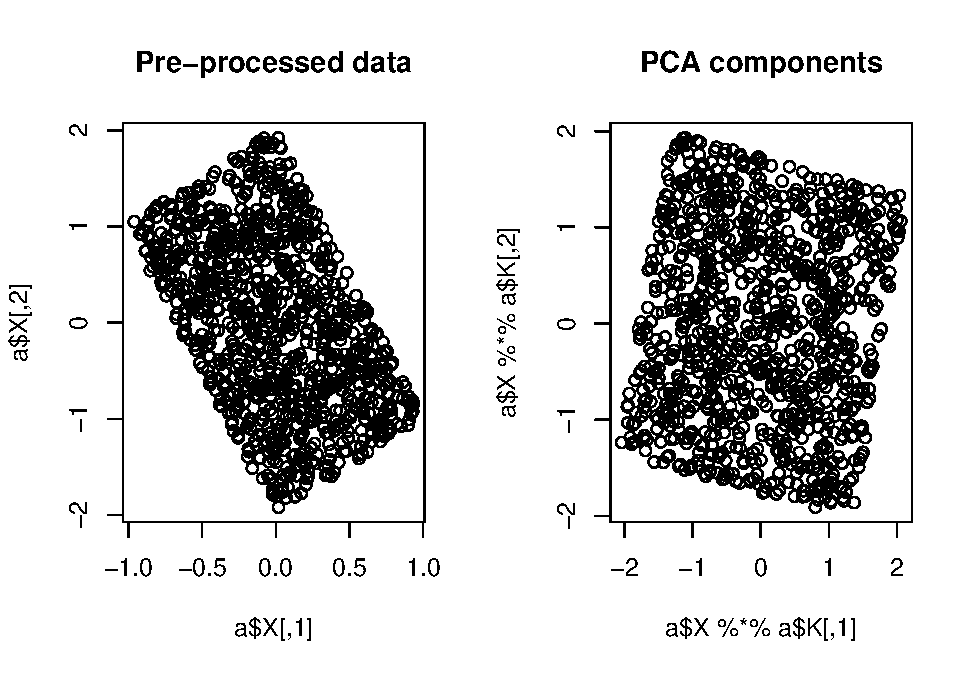
\includegraphics{ICA_Stats_Comps_files/figure-latex/unnamed-chunk-1-1} \end{center}
  
  \begin{Shaded}
  \begin{Highlighting}[]
  \KeywordTok{par}\NormalTok{(}\DataTypeTok{mfrow =} \KeywordTok{c}\NormalTok{(}\DecValTok{1}\NormalTok{, }\DecValTok{3}\NormalTok{))}
  
  \KeywordTok{plot}\NormalTok{(a}\OperatorTok{$}\NormalTok{S, }\DataTypeTok{main =} \StringTok{"ICA components fastICA"}\NormalTok{)}
  \KeywordTok{plot}\NormalTok{(b}\OperatorTok{$}\NormalTok{S,}\DataTypeTok{main=}\StringTok{"ICA Jade"}\NormalTok{)}
  \KeywordTok{plot}\NormalTok{(c}\OperatorTok{$}\NormalTok{S, }\DataTypeTok{main=}\StringTok{"ICA Infomax"}\NormalTok{)}
  \end{Highlighting}
  \end{Shaded}
  
  \begin{center}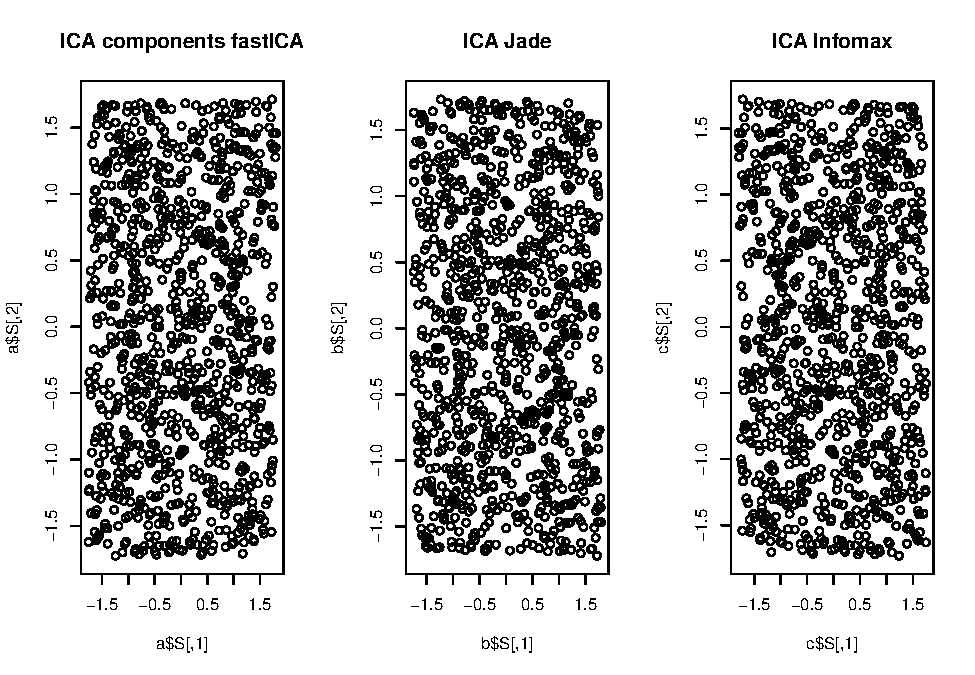
\includegraphics{ICA_Stats_Comps_files/figure-latex/unnamed-chunk-1-2} \end{center}
  
  \subsubsection{Plot Interpretation}\label{plot-interpretation}
  
  Looking at these plots, we see that the preprocessed data is rotated and
  no signals are clear from it.
  
  PCA appear to have flattened the data slightly and creates almost a
  mirror of the original data, but the true signals from the distributions
  still do not appear completely evident. PCA does not effectively
  separate sources given how it rotates data.
  
  However, looking at the ICA transformation, we can which clearly see the
  shape of a uniform distribution forming after the decomposition. ICA was
  able to recover the original signals quite easily in this simple
  simulation. The results for all 3 ICA packages (JADE,Infomax and
  fastICA) appear to produce approximately the same plots for this
  example.
  
  \subsection{(More) Complex Example: The Cocktail Party
  Problem}\label{more-complex-example-the-cocktail-party-problem}
  
  The most common example used to explain and motive the use of ICA is the
  ``Cocktail Party Problem.''
  
  Two microphones are placed in a room where to different people are
  speaking at the same time. Each microphone signal is defined as
  \(x_1(t)\) and \(x_2(t)\), with some observed (i.e.~known) amplitudes
  \(x_1\) and \(x_2\) with time as an index. The unknown speech signals by
  the speakers are \(s_1(t)\) and \(s_2(t)\) to make up the following
  system of equations:
  
  \[ x_1(t) = a_{11}s_1 +a_{12}s_2 \]
  
  \[ x_2(t) = a_{21}s_1 +a_{22}s_2 \]
  
  This can also be rewritten as:
  
  \[x_i = \begin{bmatrix} x_1 \\ x_2 \end{bmatrix}\]
  \[s_i = \begin{bmatrix} s_1 \\ s_2 \end{bmatrix}\]
  \[A = \begin{bmatrix} a_{11} & a_{12} \\ a_{21} & a_{22}  \end{bmatrix}\]
  
  If we knew the weighted \(a_{ij}\), this problem could be easily solved
  but since we do not, we must use blind source separation.
  
  \subsubsection{Example with Cocktail Party
  Data}\label{example-with-cocktail-party-data}
  
  As a test example/simulation, we can use the CPPdata from the JADE
  package that contains 50,000 observations from 4 different microphones.
  
  \begin{verbatim}
  Centering
  Whitening
  Symmetric FastICA using logcosh approx. to neg-entropy function
  Iteration 1 tol=0.047273
  Iteration 2 tol=0.007242
  Iteration 3 tol=0.000012
  \end{verbatim}
  
  \begin{verbatim}
  Warning in icajade(dat, 4, center = TRUE, maxit = 200, tol = 1e-04): Numerical rank of X is less than requested number of components (nc).
    Number of components has been redefined as the numerical rank of X.
  \end{verbatim}
  
  \begin{verbatim}
  Warning in icaimax(dat, nc = 4, center = TRUE, maxit = 200, tol = 1e-04, : Numerical rank of X is less than requested number of components (nc).
    Number of components has been redefined as the numerical rank of X.
  \end{verbatim}
  
  \begin{center}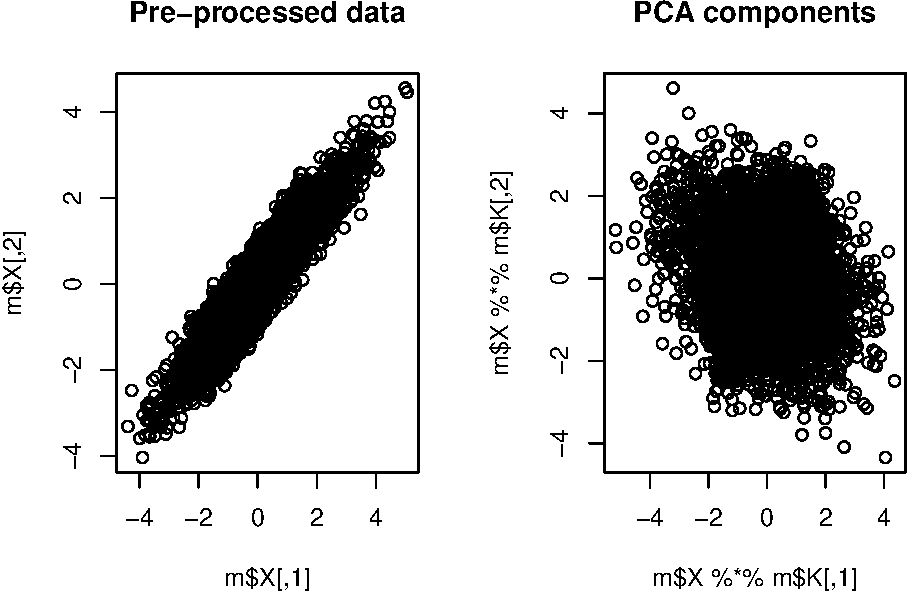
\includegraphics{ICA_Stats_Comps_files/figure-latex/unnamed-chunk-2-1} \end{center}
  
  \begin{center}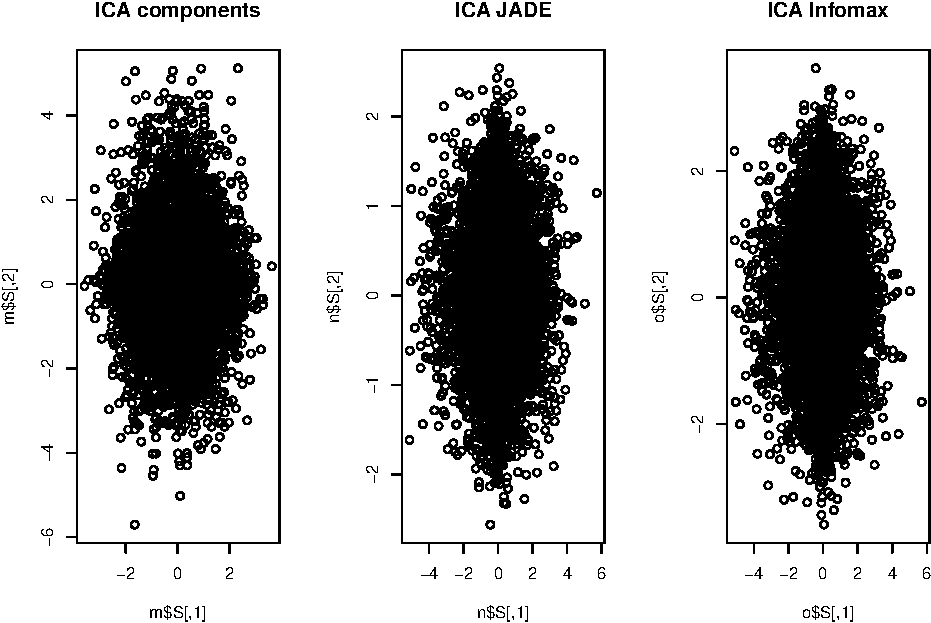
\includegraphics{ICA_Stats_Comps_files/figure-latex/unnamed-chunk-2-2} \end{center}
  
  \subsubsection{Plot Interpretation}\label{plot-interpretation-1}
  
  Again, we have a highly rotated set of pre-processed data and a PCA
  rotation that only transforms the data enough to separate the mixture
  ever so slightly.
  
  With ICA, we see a full rotation and a much cleaner shape beginning to
  form, almost diamond-like. Like with the random uniform example, the
  superior performance of any one of the three ICA methods is not
  identifible just from these primitive plots of the model.
  
  Of note with the ICA algorithms example is the ``nc'' (number of
  components) input of the function for each of these different methods.
  Particularly, both the JADE and Infomax produce similar plots at
  \(nc=4\), which makes sense as the dataset \(CPPdata\) has observations
  from 4 microphones. However, to generate a similar plot for fastICA,
  \(nc=2\) was used. The results for \(nc=4\) with ICA appear as below
  (JADE and Infomax shown at \(nc=2\) for reverse comparison:
  
  \begin{Shaded}
  \begin{Highlighting}[]
  \KeywordTok{set.seed}\NormalTok{(}\DecValTok{10}\NormalTok{)}
  \KeywordTok{library}\NormalTok{(fastICA)}
  \NormalTok{S <-}\StringTok{ }\KeywordTok{matrix}\NormalTok{(}\KeywordTok{runif}\NormalTok{(}\DecValTok{10000}\NormalTok{), }\DecValTok{1000}\NormalTok{, }\DecValTok{2}\NormalTok{)}
  \NormalTok{A <-}\StringTok{ }\KeywordTok{matrix}\NormalTok{(}\KeywordTok{c}\NormalTok{(}\DecValTok{1}\NormalTok{, }\DecValTok{1}\NormalTok{, }\OperatorTok{-}\DecValTok{1}\NormalTok{, }\DecValTok{3}\NormalTok{), }\DecValTok{2}\NormalTok{, }\DecValTok{2}\NormalTok{, }\DataTypeTok{byrow =} \OtherTok{TRUE}\NormalTok{)}
  \NormalTok{X <-}\StringTok{ }\NormalTok{S }\OperatorTok\StringTok{ }\NormalTok{A}
  \NormalTok{m <-}\StringTok{ }\KeywordTok{fastICA}\NormalTok{(dat,}\DecValTok{4}\NormalTok{,}\DataTypeTok{alg.typ =} \StringTok{"parallel"}\NormalTok{, }\DataTypeTok{fun =} \StringTok{"logcosh"}\NormalTok{, }\DataTypeTok{alpha =} \DecValTok{1}\NormalTok{, }
               \DataTypeTok{method =} \StringTok{"C"}\NormalTok{, }\DataTypeTok{row.norm =} \OtherTok{FALSE}\NormalTok{, }\DataTypeTok{maxit =} \DecValTok{200}\NormalTok{, }
               \DataTypeTok{tol =} \FloatTok{0.0001}\NormalTok{, }\DataTypeTok{verbose =} \OtherTok{TRUE}\NormalTok{)}
  \end{Highlighting}
  \end{Shaded}
  
  \begin{verbatim}
  Centering
  Whitening
  Symmetric FastICA using logcosh approx. to neg-entropy function
  Iteration 1 tol=0.380613
  Iteration 2 tol=0.254897
  Iteration 3 tol=0.146511
  Iteration 4 tol=0.072136
  Iteration 5 tol=0.031287
  Iteration 6 tol=0.012479
  Iteration 7 tol=0.004745
  Iteration 8 tol=0.001764
  Iteration 9 tol=0.000650
  Iteration 10 tol=0.000238
  Iteration 11 tol=0.000087
  \end{verbatim}
  
  \begin{Shaded}
  \begin{Highlighting}[]
  \NormalTok{n <-}\StringTok{ }\KeywordTok{icajade}\NormalTok{(dat,}\DecValTok{2}\NormalTok{,}\DataTypeTok{center=}\OtherTok{TRUE}\NormalTok{,}\DataTypeTok{maxit=}\DecValTok{200}\NormalTok{,}\DataTypeTok{tol=}\FloatTok{0.0001}\NormalTok{)}
  
  \NormalTok{o <-}\StringTok{ }\KeywordTok{icaimax}\NormalTok{(dat,}\DataTypeTok{nc=}\DecValTok{2}\NormalTok{,}\DataTypeTok{center=}\OtherTok{TRUE}\NormalTok{,}\DataTypeTok{maxit=}\DecValTok{200}\NormalTok{,}\DataTypeTok{tol=}\FloatTok{0.0001}\NormalTok{,}\DataTypeTok{alg=}\StringTok{"newton"}\NormalTok{,}\DataTypeTok{fun=}\StringTok{"log"}\NormalTok{)}
  
  \KeywordTok{par}\NormalTok{(}\DataTypeTok{mfrow =} \KeywordTok{c}\NormalTok{(}\DecValTok{1}\NormalTok{,}\DecValTok{3}\NormalTok{))}
  \KeywordTok{plot}\NormalTok{(m}\OperatorTok{$}\NormalTok{S, }\DataTypeTok{main =} \StringTok{"ICA components"}\NormalTok{)}
  \KeywordTok{plot}\NormalTok{(n}\OperatorTok{$}\NormalTok{S, }\DataTypeTok{main =} \StringTok{"ICA JADE"}\NormalTok{)}
  \KeywordTok{plot}\NormalTok{(o}\OperatorTok{$}\NormalTok{S, }\DataTypeTok{main =}\StringTok{"ICA Infomax"}\NormalTok{)}
  \end{Highlighting}
  \end{Shaded}
  
  \begin{center}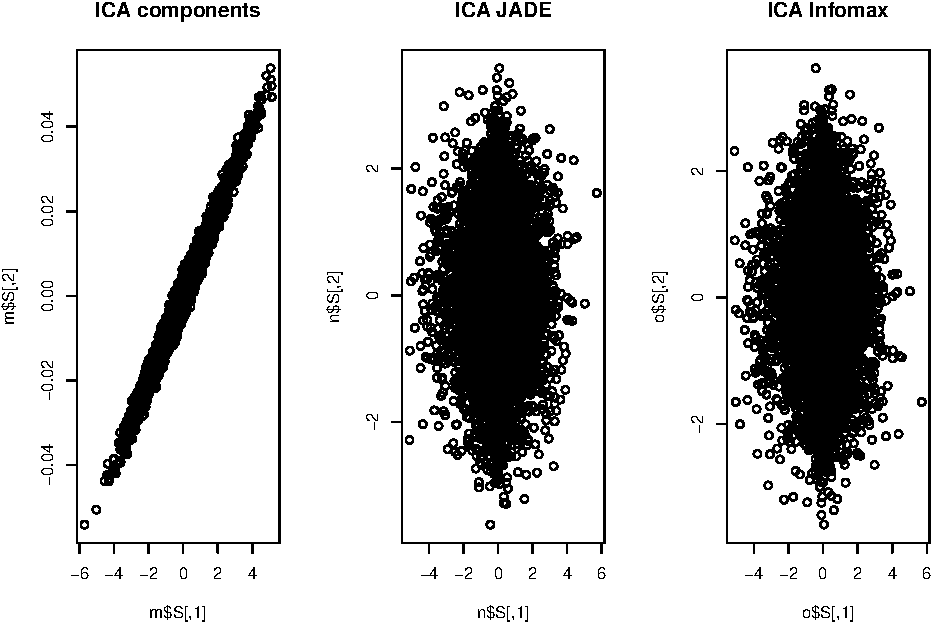
\includegraphics{ICA_Stats_Comps_files/figure-latex/unnamed-chunk-3-1} \end{center}
  
  While JADE and Infomax at \(nc=2\) do not differ greatly from \(nc=4\),
  the fastICA plot appears more similar to the pre-processed data when the
  number of components is set at 4.
  
  \paragraph{Explain what this could
  mean}\label{explain-what-this-could-mean}
  
  \section{Simulation}\label{simulation}
  
  Given the simplistic nature of both toy examples, a simulation can
  provide more robust insight into the effectiveness of ICA in extracting
  original source components.
  
  For this, we will use the Monte Carlo Markov Chain (MCMC) and see how
  ICA performs in a ``noisier'' setting.
  
  \subsection{Random Uniform
  Distribution}\label{random-uniform-distribution}
  
  \begin{Shaded}
  \begin{Highlighting}[]
  \NormalTok{a <-}\StringTok{ }\KeywordTok{fastICA}\NormalTok{(X, }\DecValTok{2}\NormalTok{, }\DataTypeTok{alg.typ =} \StringTok{"parallel"}\NormalTok{, }\DataTypeTok{fun =} \StringTok{"logcosh"}\NormalTok{, }\DataTypeTok{alpha =} \DecValTok{1}\NormalTok{, }
               \DataTypeTok{method =} \StringTok{"C"}\NormalTok{, }\DataTypeTok{row.norm =} \OtherTok{FALSE}\NormalTok{, }\DataTypeTok{maxit =} \DecValTok{200}\NormalTok{, }
               \DataTypeTok{tol =} \FloatTok{0.0001}\NormalTok{, }\DataTypeTok{verbose =} \OtherTok{TRUE}\NormalTok{)}
  \end{Highlighting}
  \end{Shaded}
  
  \begin{verbatim}
  Centering
  Whitening
  Symmetric FastICA using logcosh approx. to neg-entropy function
  Iteration 1 tol=0.116217
  Iteration 2 tol=0.000607
  Iteration 3 tol=0.000007
  \end{verbatim}
  
  \begin{Shaded}
  \begin{Highlighting}[]
  \NormalTok{b <-}\StringTok{ }\KeywordTok{icajade}\NormalTok{(X,}\DecValTok{2}\NormalTok{,}\DataTypeTok{center=}\OtherTok{TRUE}\NormalTok{,}\DataTypeTok{maxit=}\DecValTok{200}\NormalTok{,}\DataTypeTok{tol=}\FloatTok{0.0001}\NormalTok{)}
  
  \NormalTok{c <-}\StringTok{ }\KeywordTok{icaimax}\NormalTok{(X,}\DataTypeTok{nc=}\DecValTok{2}\NormalTok{,}\DataTypeTok{center=}\OtherTok{TRUE}\NormalTok{,}\DataTypeTok{maxit=}\DecValTok{200}\NormalTok{,}\DataTypeTok{tol=}\FloatTok{0.0001}\NormalTok{,}\DataTypeTok{alg=}\StringTok{"newton"}\NormalTok{,}\DataTypeTok{fun=}\StringTok{"log"}\NormalTok{)}
  
  \KeywordTok{par}\NormalTok{(}\DataTypeTok{mfrow =} \KeywordTok{c}\NormalTok{(}\DecValTok{1}\NormalTok{, }\DecValTok{2}\NormalTok{))}
  \KeywordTok{plot}\NormalTok{(a}\OperatorTok{$}\NormalTok{X, }\DataTypeTok{main =} \StringTok{"Pre-processed data"}\NormalTok{)}
  \KeywordTok{plot}\NormalTok{(a}\OperatorTok{$}\NormalTok{X }\OperatorTok\StringTok{ }\NormalTok{a}\OperatorTok{$}\NormalTok{K, }\DataTypeTok{main =} \StringTok{"PCA components"}\NormalTok{)}
  \end{Highlighting}
  \end{Shaded}
  
  \begin{center}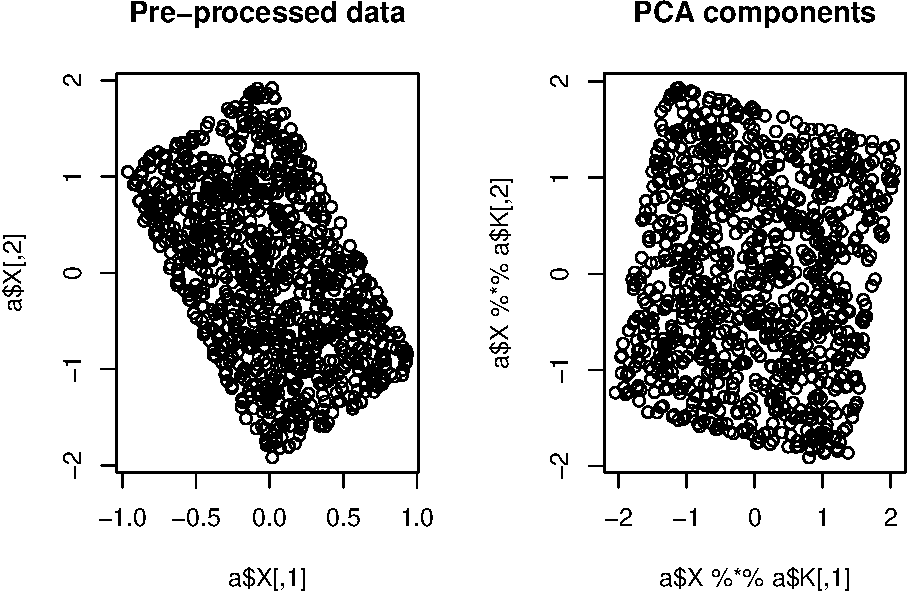
\includegraphics{ICA_Stats_Comps_files/figure-latex/unnamed-chunk-4-1} \end{center}
  
  \begin{Shaded}
  \begin{Highlighting}[]
  \KeywordTok{par}\NormalTok{(}\DataTypeTok{mfrow =} \KeywordTok{c}\NormalTok{(}\DecValTok{1}\NormalTok{, }\DecValTok{3}\NormalTok{))}
  
  \KeywordTok{plot}\NormalTok{(a}\OperatorTok{$}\NormalTok{S, }\DataTypeTok{main =} \StringTok{"ICA components fastICA"}\NormalTok{)}
  \KeywordTok{plot}\NormalTok{(b}\OperatorTok{$}\NormalTok{S,}\DataTypeTok{main=}\StringTok{"ICA Jade"}\NormalTok{)}
  \KeywordTok{plot}\NormalTok{(c}\OperatorTok{$}\NormalTok{S, }\DataTypeTok{main=}\StringTok{"ICA Infomax"}\NormalTok{)}
  \end{Highlighting}
  \end{Shaded}
  
  \begin{center}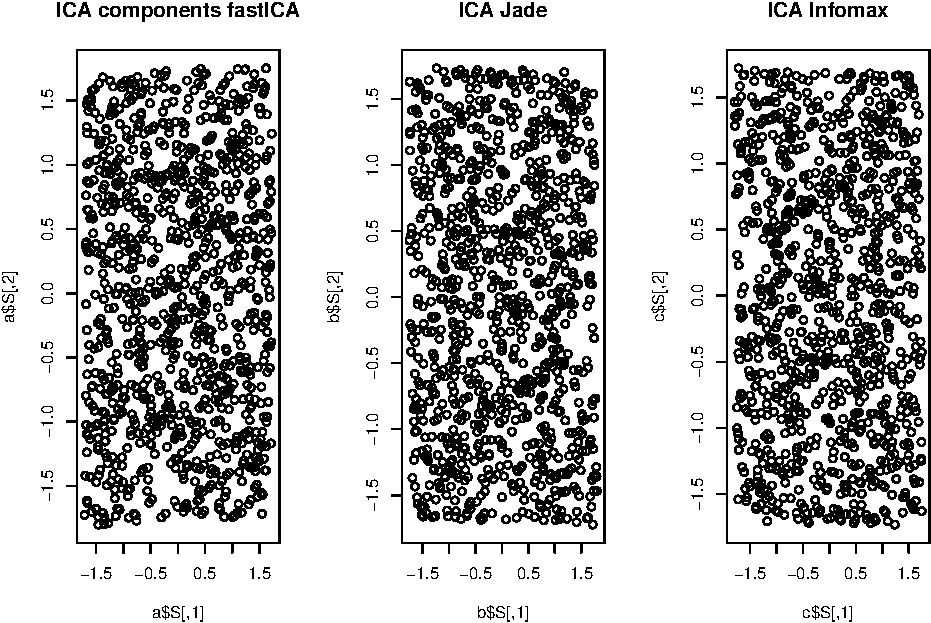
\includegraphics{ICA_Stats_Comps_files/figure-latex/unnamed-chunk-4-2} \end{center}
  
  \section{CPP Simulation}\label{cpp-simulation}
  
  \begin{Shaded}
  \begin{Highlighting}[]
  \NormalTok{m <-}\StringTok{ }\KeywordTok{fastICA}\NormalTok{(r1,}\DecValTok{2}\NormalTok{,}\DataTypeTok{alg.typ =} \StringTok{"parallel"}\NormalTok{, }\DataTypeTok{fun =} \StringTok{"logcosh"}\NormalTok{, }\DataTypeTok{alpha =} \DecValTok{1}\NormalTok{, }
               \DataTypeTok{method =} \StringTok{"C"}\NormalTok{, }\DataTypeTok{row.norm =} \OtherTok{FALSE}\NormalTok{, }\DataTypeTok{maxit =} \DecValTok{200}\NormalTok{, }
               \DataTypeTok{tol =} \FloatTok{0.0001}\NormalTok{, }\DataTypeTok{verbose =} \OtherTok{TRUE}\NormalTok{)}
  \end{Highlighting}
  \end{Shaded}
  
  \begin{verbatim}
  Centering
  Whitening
  Symmetric FastICA using logcosh approx. to neg-entropy function
  Iteration 1 tol=0.006395
  Iteration 2 tol=0.000040
  \end{verbatim}
  
  \begin{Shaded}
  \begin{Highlighting}[]
  \NormalTok{n <-}\StringTok{ }\KeywordTok{icajade}\NormalTok{(r1,}\DecValTok{2}\NormalTok{,}\DataTypeTok{center=}\OtherTok{TRUE}\NormalTok{,}\DataTypeTok{maxit=}\DecValTok{200}\NormalTok{,}\DataTypeTok{tol=}\FloatTok{0.0001}\NormalTok{)}
  
  \NormalTok{o <-}\StringTok{ }\KeywordTok{icaimax}\NormalTok{(r1,}\DataTypeTok{nc=}\DecValTok{2}\NormalTok{,}\DataTypeTok{center=}\OtherTok{TRUE}\NormalTok{,}\DataTypeTok{maxit=}\DecValTok{200}\NormalTok{,}\DataTypeTok{tol=}\FloatTok{0.0001}\NormalTok{,}\DataTypeTok{alg=}\StringTok{"newton"}\NormalTok{,}\DataTypeTok{fun=}\StringTok{"log"}\NormalTok{)}
  
  \KeywordTok{par}\NormalTok{(}\DataTypeTok{mfrow =} \KeywordTok{c}\NormalTok{(}\DecValTok{1}\NormalTok{,}\DecValTok{2}\NormalTok{))}
  \KeywordTok{plot}\NormalTok{(m}\OperatorTok{$}\NormalTok{X, }\DataTypeTok{main =} \StringTok{"Pre-processed data"}\NormalTok{)}
  \KeywordTok{plot}\NormalTok{(m}\OperatorTok{$}\NormalTok{X }\OperatorTok\StringTok{ }\NormalTok{m}\OperatorTok{$}\NormalTok{K, }\DataTypeTok{main =} \StringTok{"PCA components"}\NormalTok{)}
  \end{Highlighting}
  \end{Shaded}
  
  \begin{center}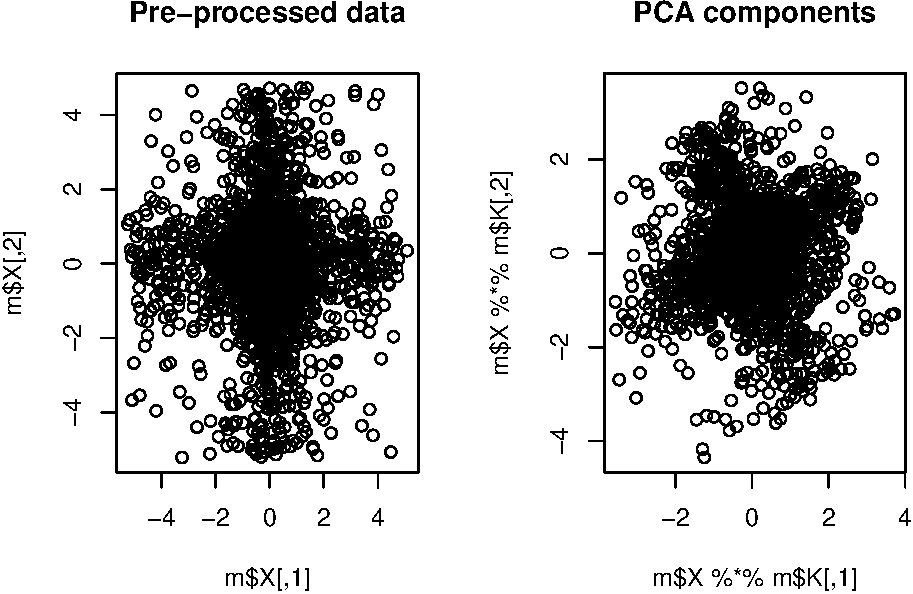
\includegraphics{ICA_Stats_Comps_files/figure-latex/unnamed-chunk-6-1} \end{center}
  
  \begin{Shaded}
  \begin{Highlighting}[]
  \KeywordTok{par}\NormalTok{(}\DataTypeTok{mfrow =} \KeywordTok{c}\NormalTok{(}\DecValTok{1}\NormalTok{,}\DecValTok{3}\NormalTok{))}
  
  \KeywordTok{plot}\NormalTok{(m}\OperatorTok{$}\NormalTok{S, }\DataTypeTok{main =} \StringTok{"ICA components"}\NormalTok{)}
  \KeywordTok{plot}\NormalTok{(n}\OperatorTok{$}\NormalTok{S, }\DataTypeTok{main =} \StringTok{"ICA JADE"}\NormalTok{)}
  \KeywordTok{plot}\NormalTok{(o}\OperatorTok{$}\NormalTok{S, }\DataTypeTok{main =}\StringTok{"ICA Infomax"}\NormalTok{)}
  \end{Highlighting}
  \end{Shaded}
  
  \begin{center}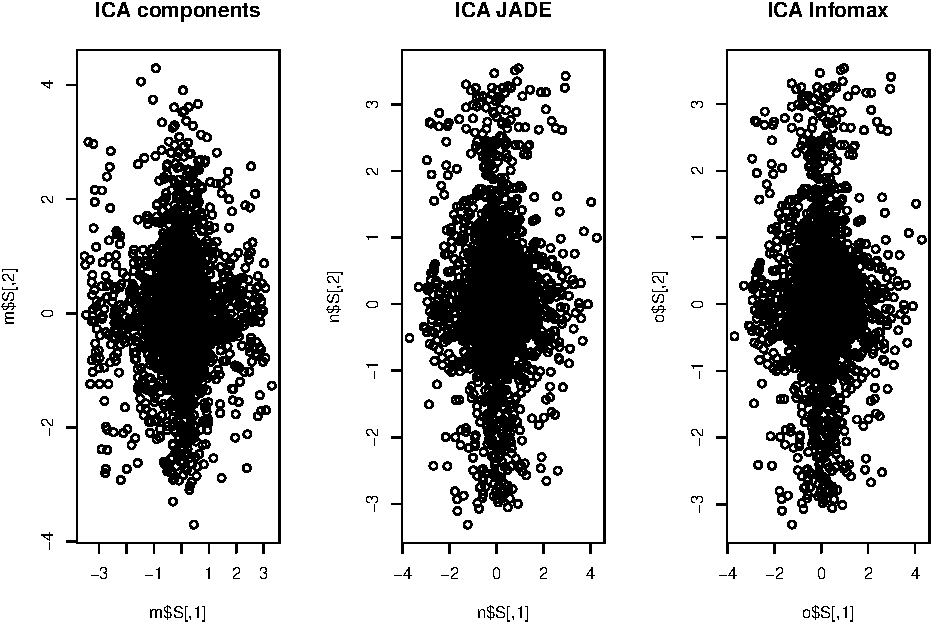
\includegraphics{ICA_Stats_Comps_files/figure-latex/unnamed-chunk-6-2} \end{center}
  
  \begin{Shaded}
  \begin{Highlighting}[]
  \NormalTok{m <-}\StringTok{ }\KeywordTok{fastICA}\NormalTok{(r2,}\DecValTok{2}\NormalTok{,}\DataTypeTok{alg.typ =} \StringTok{"parallel"}\NormalTok{, }\DataTypeTok{fun =} \StringTok{"logcosh"}\NormalTok{, }\DataTypeTok{alpha =} \DecValTok{1}\NormalTok{, }
               \DataTypeTok{method =} \StringTok{"C"}\NormalTok{, }\DataTypeTok{row.norm =} \OtherTok{FALSE}\NormalTok{, }\DataTypeTok{maxit =} \DecValTok{200}\NormalTok{, }
               \DataTypeTok{tol =} \FloatTok{0.0001}\NormalTok{, }\DataTypeTok{verbose =} \OtherTok{TRUE}\NormalTok{)}
  \end{Highlighting}
  \end{Shaded}
  
  \begin{verbatim}
  Centering
  Whitening
  Symmetric FastICA using logcosh approx. to neg-entropy function
  Iteration 1 tol=0.022903
  Iteration 2 tol=0.002771
  Iteration 3 tol=0.000168
  Iteration 4 tol=0.000008
  \end{verbatim}
  
  \begin{Shaded}
  \begin{Highlighting}[]
  \NormalTok{n <-}\StringTok{ }\KeywordTok{icajade}\NormalTok{(r2,}\DecValTok{2}\NormalTok{,}\DataTypeTok{center=}\OtherTok{TRUE}\NormalTok{,}\DataTypeTok{maxit=}\DecValTok{200}\NormalTok{,}\DataTypeTok{tol=}\FloatTok{0.0001}\NormalTok{)}
  
  \NormalTok{o <-}\StringTok{ }\KeywordTok{icaimax}\NormalTok{(r2,}\DataTypeTok{nc=}\DecValTok{2}\NormalTok{,}\DataTypeTok{center=}\OtherTok{TRUE}\NormalTok{,}\DataTypeTok{maxit=}\DecValTok{200}\NormalTok{,}\DataTypeTok{tol=}\FloatTok{0.0001}\NormalTok{,}\DataTypeTok{alg=}\StringTok{"newton"}\NormalTok{,}\DataTypeTok{fun=}\StringTok{"log"}\NormalTok{)}
  
  \KeywordTok{par}\NormalTok{(}\DataTypeTok{mfrow =} \KeywordTok{c}\NormalTok{(}\DecValTok{1}\NormalTok{,}\DecValTok{2}\NormalTok{))}
  \KeywordTok{plot}\NormalTok{(m}\OperatorTok{$}\NormalTok{X, }\DataTypeTok{main =} \StringTok{"Pre-processed data"}\NormalTok{)}
  \KeywordTok{plot}\NormalTok{(m}\OperatorTok{$}\NormalTok{X }\OperatorTok\StringTok{ }\NormalTok{m}\OperatorTok{$}\NormalTok{K, }\DataTypeTok{main =} \StringTok{"PCA components"}\NormalTok{)}
  \end{Highlighting}
  \end{Shaded}
  
  \begin{center}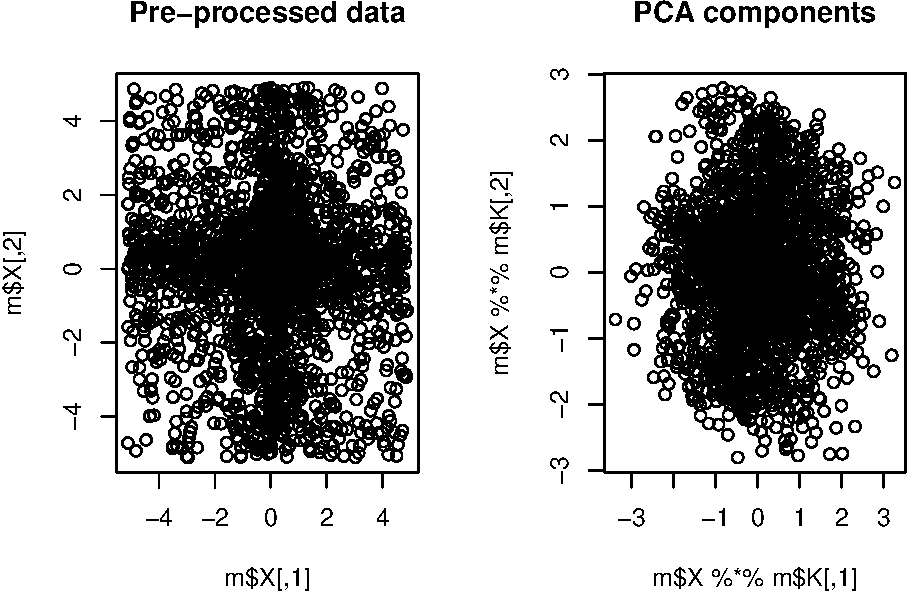
\includegraphics{ICA_Stats_Comps_files/figure-latex/unnamed-chunk-7-1} \end{center}
  
  \begin{Shaded}
  \begin{Highlighting}[]
  \KeywordTok{par}\NormalTok{(}\DataTypeTok{mfrow =} \KeywordTok{c}\NormalTok{(}\DecValTok{1}\NormalTok{,}\DecValTok{3}\NormalTok{))}
  
  \KeywordTok{plot}\NormalTok{(m}\OperatorTok{$}\NormalTok{S, }\DataTypeTok{main =} \StringTok{"ICA components"}\NormalTok{)}
  \KeywordTok{plot}\NormalTok{(n}\OperatorTok{$}\NormalTok{S, }\DataTypeTok{main =} \StringTok{"ICA JADE"}\NormalTok{)}
  \KeywordTok{plot}\NormalTok{(o}\OperatorTok{$}\NormalTok{S, }\DataTypeTok{main =}\StringTok{"ICA Infomax"}\NormalTok{)}
  \end{Highlighting}
  \end{Shaded}
  
  \begin{center}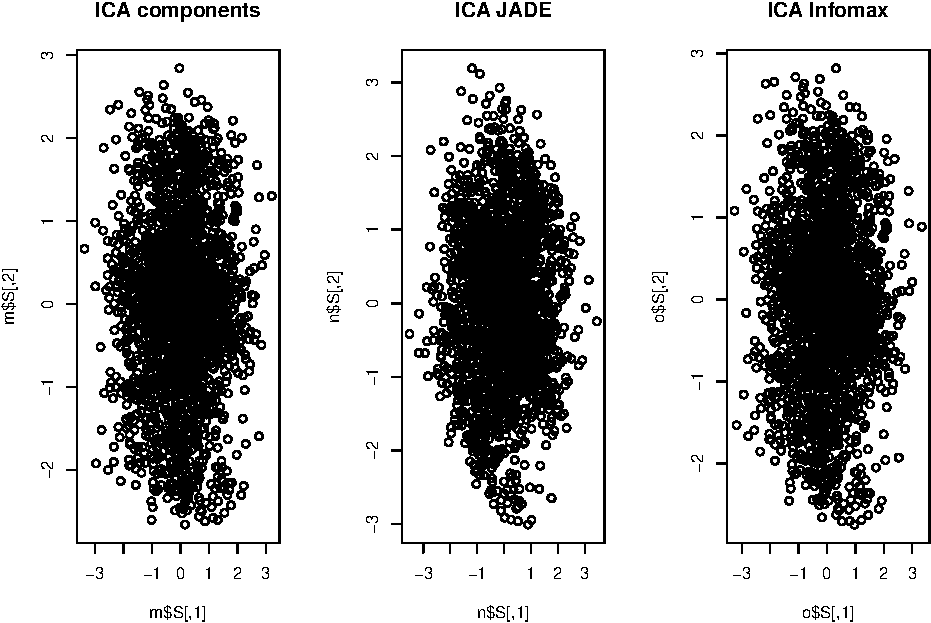
\includegraphics{ICA_Stats_Comps_files/figure-latex/unnamed-chunk-7-2} \end{center}
  
  \begin{Shaded}
  \begin{Highlighting}[]
  \NormalTok{m <-}\StringTok{ }\KeywordTok{fastICA}\NormalTok{(r3,}\DecValTok{2}\NormalTok{,}\DataTypeTok{alg.typ =} \StringTok{"parallel"}\NormalTok{, }\DataTypeTok{fun =} \StringTok{"logcosh"}\NormalTok{, }\DataTypeTok{alpha =} \DecValTok{1}\NormalTok{, }
               \DataTypeTok{method =} \StringTok{"C"}\NormalTok{, }\DataTypeTok{row.norm =} \OtherTok{FALSE}\NormalTok{, }\DataTypeTok{maxit =} \DecValTok{200}\NormalTok{, }
               \DataTypeTok{tol =} \FloatTok{0.0001}\NormalTok{, }\DataTypeTok{verbose =} \OtherTok{TRUE}\NormalTok{)}
  \end{Highlighting}
  \end{Shaded}
  
  \begin{verbatim}
  Centering
  Whitening
  Symmetric FastICA using logcosh approx. to neg-entropy function
  Iteration 1 tol=0.050045
  Iteration 2 tol=0.014569
  Iteration 3 tol=0.000013
  \end{verbatim}
  
  \begin{Shaded}
  \begin{Highlighting}[]
  \NormalTok{n <-}\StringTok{ }\KeywordTok{icajade}\NormalTok{(r3,}\DecValTok{2}\NormalTok{,}\DataTypeTok{center=}\OtherTok{TRUE}\NormalTok{,}\DataTypeTok{maxit=}\DecValTok{200}\NormalTok{,}\DataTypeTok{tol=}\FloatTok{0.0001}\NormalTok{)}
  
  \NormalTok{o <-}\StringTok{ }\KeywordTok{icaimax}\NormalTok{(r3,}\DataTypeTok{nc=}\DecValTok{2}\NormalTok{,}\DataTypeTok{center=}\OtherTok{TRUE}\NormalTok{,}\DataTypeTok{maxit=}\DecValTok{200}\NormalTok{,}\DataTypeTok{tol=}\FloatTok{0.0001}\NormalTok{,}\DataTypeTok{alg=}\StringTok{"newton"}\NormalTok{,}\DataTypeTok{fun=}\StringTok{"log"}\NormalTok{)}
  
  \KeywordTok{par}\NormalTok{(}\DataTypeTok{mfrow =} \KeywordTok{c}\NormalTok{(}\DecValTok{1}\NormalTok{,}\DecValTok{2}\NormalTok{))}
  \KeywordTok{plot}\NormalTok{(m}\OperatorTok{$}\NormalTok{X, }\DataTypeTok{main =} \StringTok{"Pre-processed data"}\NormalTok{)}
  \KeywordTok{plot}\NormalTok{(m}\OperatorTok{$}\NormalTok{X }\OperatorTok\StringTok{ }\NormalTok{m}\OperatorTok{$}\NormalTok{K, }\DataTypeTok{main =} \StringTok{"PCA components"}\NormalTok{)}
  \end{Highlighting}
  \end{Shaded}
  
  \begin{center}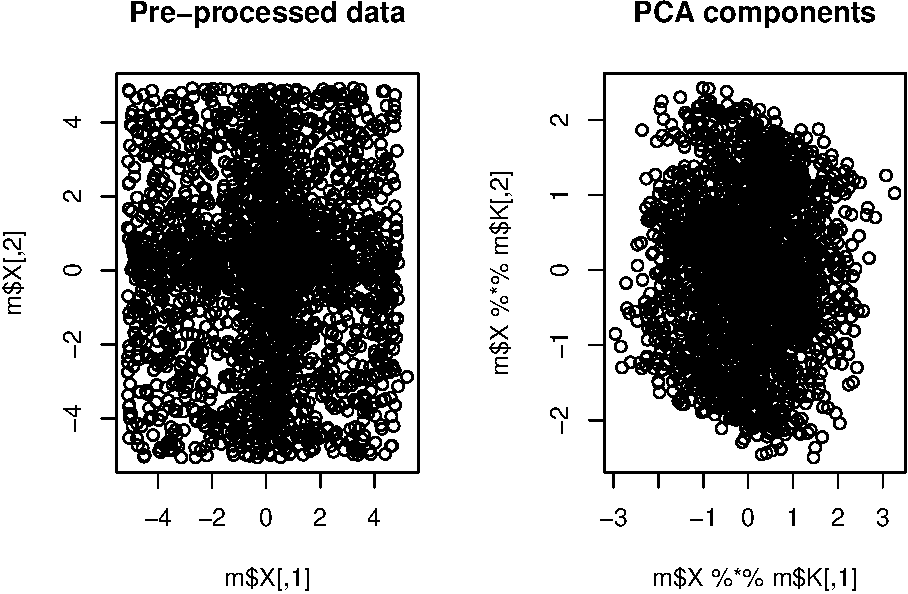
\includegraphics{ICA_Stats_Comps_files/figure-latex/unnamed-chunk-8-1} \end{center}
  
  \begin{Shaded}
  \begin{Highlighting}[]
  \KeywordTok{par}\NormalTok{(}\DataTypeTok{mfrow =} \KeywordTok{c}\NormalTok{(}\DecValTok{1}\NormalTok{,}\DecValTok{3}\NormalTok{))}
  
  \KeywordTok{plot}\NormalTok{(m}\OperatorTok{$}\NormalTok{S, }\DataTypeTok{main =} \StringTok{"ICA components"}\NormalTok{)}
  \KeywordTok{plot}\NormalTok{(n}\OperatorTok{$}\NormalTok{S, }\DataTypeTok{main =} \StringTok{"ICA JADE"}\NormalTok{)}
  \KeywordTok{plot}\NormalTok{(o}\OperatorTok{$}\NormalTok{S, }\DataTypeTok{main =}\StringTok{"ICA Infomax"}\NormalTok{)}
  \end{Highlighting}
  \end{Shaded}
  
  \begin{center}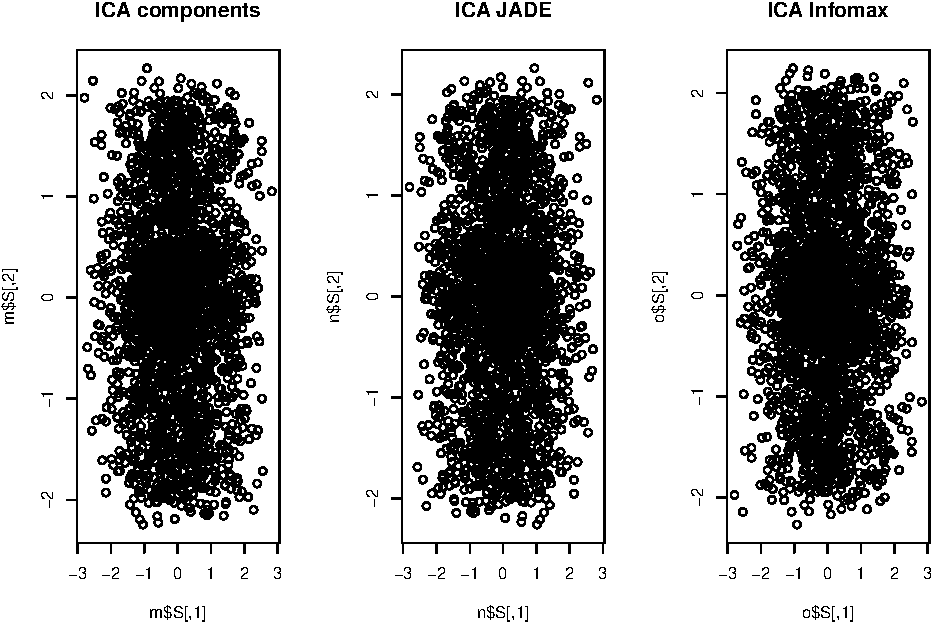
\includegraphics{ICA_Stats_Comps_files/figure-latex/unnamed-chunk-8-2} \end{center}
  
  \chapter{Computation and Application to
  Dataset}\label{computation-and-application-to-dataset}
  
  \section{The Dataset: Walmart Store Data from
  Kaggle}\label{the-dataset-walmart-store-data-from-kaggle}
  
  From a 2014 Kaggle competition in attempt to forecast sales , the
  Walmart Store dataset provides information on sales for \(n=45\) located
  in different regions of the United States. Each store has Weekly Sales
  data from \(2010-02-05\) to \(2012-11-01\), information by department
  and a binary IsHoliday variable.
  
  \subsection{Prior Analysis : Kimmo Kiviluoto and Erkki
  Oja}\label{prior-analysis-kimmo-kiviluoto-and-erkki-oja}
  
  In 1998, Kiviluoto and Erkki Oja used ICA on parallel Financial Time
  Series from a retail chain of 40 stores. They claim in their paper
  \textit{Independent Comp onent Analysis for Parallel Financial Time Series}
  that by removing the fundamental factors of the data, they were able to
  see the impact of management decisions of a particular store more
  clearly.
  
  With the walmart store data, an attempt to show a similar result using
  retail data will be made. However, this will look at weekly sales not
  cashflow data, which will probably not generate as robust results since
  cashflow provides more information about financial activities than just
  sales.
  
  \subsection{Exploration}\label{exploration}
  
  \section{FastICA Algorithm}\label{fastica-algorithm}
  
  \section{FastICA
  Application/Simulation}\label{fastica-applicationsimulation}
  
  \begin{Shaded}
  \begin{Highlighting}[]
  \NormalTok{a <-}\KeywordTok{fastICA}\NormalTok{(w2,}\DecValTok{3}\NormalTok{, }\DataTypeTok{alg.typ=}\StringTok{"parallel"}\NormalTok{,}\DataTypeTok{fun=} \StringTok{"logcosh"}\NormalTok{,,}\DataTypeTok{row.norm=}\OtherTok{FALSE}\NormalTok{,}\DataTypeTok{maxit=}\DecValTok{5}\NormalTok{,}\DataTypeTok{tol=} \FloatTok{0.0001}\NormalTok{,}\DataTypeTok{verbose=}\OtherTok{TRUE}\NormalTok{)}
  \end{Highlighting}
  \end{Shaded}
  
  \begin{verbatim}
  Centering
  \end{verbatim}
  
  \begin{verbatim}
  Whitening
  \end{verbatim}
  
  \begin{verbatim}
  Symmetric FastICA using logcosh approx. to neg-entropy function
  \end{verbatim}
  
  \begin{verbatim}
  Iteration 1 tol = 0.1452916
  \end{verbatim}
  
  \begin{verbatim}
  Iteration 2 tol = 0.2135624
  \end{verbatim}
  
  \begin{verbatim}
  Iteration 3 tol = 0.3292911
  \end{verbatim}
  
  \begin{verbatim}
  Iteration 4 tol = 0.5126155
  \end{verbatim}
  
  \begin{Shaded}
  \begin{Highlighting}[]
  \KeywordTok{par}\NormalTok{(}\DataTypeTok{mfrow =} \KeywordTok{c}\NormalTok{(}\DecValTok{1}\NormalTok{, }\DecValTok{3}\NormalTok{))}
  \KeywordTok{plot}\NormalTok{(a}\OperatorTok{$}\NormalTok{X, }\DataTypeTok{main =} \StringTok{"Pre-processed data"}\NormalTok{)}
  \KeywordTok{plot}\NormalTok{(a}\OperatorTok{$}\NormalTok{X }\OperatorTok\StringTok{ }\NormalTok{a}\OperatorTok{$}\NormalTok{K, }\DataTypeTok{main =} \StringTok{"PCA components"}\NormalTok{ )}
  \KeywordTok{plot}\NormalTok{(a}\OperatorTok{$}\NormalTok{S, }\DataTypeTok{main =} \StringTok{"ICA components"}\NormalTok{)  }
  \end{Highlighting}
  \end{Shaded}
  
  \begin{center}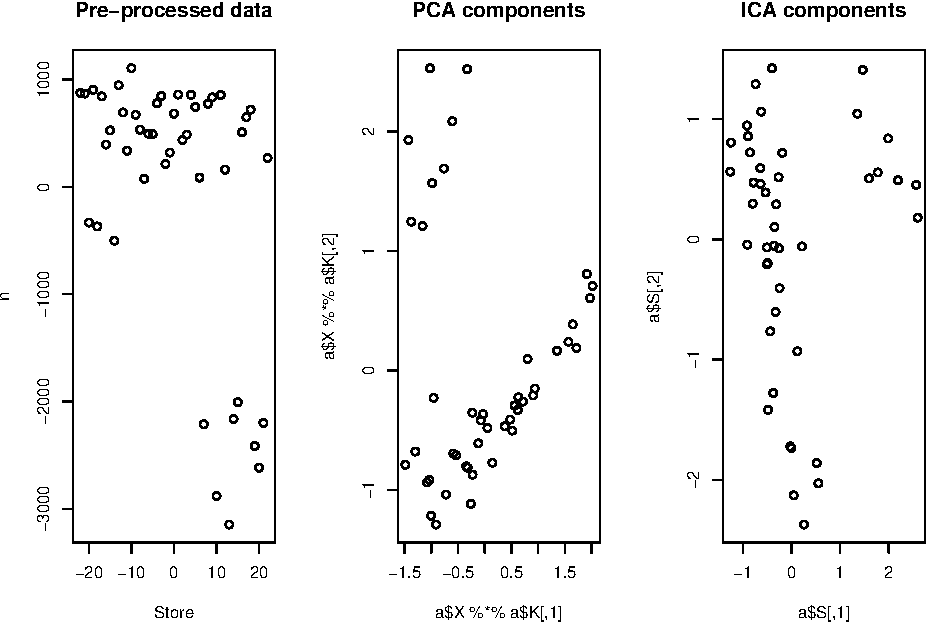
\includegraphics{ICA_Stats_Comps_files/figure-latex/unnamed-chunk-10-1} \end{center}
  
  \begin{Shaded}
  \begin{Highlighting}[]
  \NormalTok{bank <-}\StringTok{ }\KeywordTok{read_csv}\NormalTok{(}\StringTok{"bank-full.csv"}\NormalTok{)}
  \end{Highlighting}
  \end{Shaded}
  
  \begin{verbatim}
  Parsed with column specification:
  cols(
    `age";"job";"marital";"education";"default";"balance";"housing";"loan";"contact";"day";"month";"duration";"campaign";"pdays";"previous";"poutcome";"y` = col_character()
  )
  \end{verbatim}
  
  \section{Comparison to other Methods for ICA and for other
  BSS}\label{comparison-to-other-methods-for-ica-and-for-other-bss}
  
  \chapter{Visualization}\label{visualization}
  
  \section{Shiny App: Comparison of
  Methods}\label{shiny-app-comparison-of-methods}
  
  \section{Summary of Performance from
  App}\label{summary-of-performance-from-app}
  
  \subsection{ICA}\label{ica}
  
  \subsection{PCA}\label{pca}
  
  \subsection{Sparse Component Analysis
  (SCA)}\label{sparse-component-analysis-sca}
  
  \subsection{Non-negative Matrix Factorization
  (NMF)}\label{non-negative-matrix-factorization-nmf}
  
  \chapter{}\label{section}
  
  \section{Tables}\label{tables}
  
  In addition to the tables that can be automatically generated from a
  data frame in \textbf{R} that you saw in {[}R Markdown Basics{]} using
  the \texttt{kable} function, you can also create tables using
  \emph{pandoc}. (More information is available at
  \url{http://pandoc.org/README.html\#tables}.) This might be useful if
  you don't have values specifically stored in \textbf{R}, but you'd like
  to display them in table form. Below is an example. Pay careful
  attention to the alignment in the table and the use of the hyphens to
  create the rows and columns.
  
  \begin{longtable}[]{@{}ccc@{}}
  \caption{Correlation of Inheritance Factors for Parents and Child
  \label{tab:inher}}\tabularnewline
  \toprule
  \begin{minipage}[b]{0.29\columnwidth}\centering\strut
  Factors\strut
  \end{minipage} & \begin{minipage}[b]{0.47\columnwidth}\centering\strut
  Correlation between Parents \& Child\strut
  \end{minipage} & \begin{minipage}[b]{0.16\columnwidth}\centering\strut
  Inherited\strut
  \end{minipage}\tabularnewline
  \midrule
  \endfirsthead
  \toprule
  \begin{minipage}[b]{0.29\columnwidth}\centering\strut
  Factors\strut
  \end{minipage} & \begin{minipage}[b]{0.47\columnwidth}\centering\strut
  Correlation between Parents \& Child\strut
  \end{minipage} & \begin{minipage}[b]{0.16\columnwidth}\centering\strut
  Inherited\strut
  \end{minipage}\tabularnewline
  \midrule
  \endhead
  \begin{minipage}[t]{0.29\columnwidth}\centering\strut
  Education\strut
  \end{minipage} & \begin{minipage}[t]{0.47\columnwidth}\centering\strut
  -0.49\strut
  \end{minipage} & \begin{minipage}[t]{0.16\columnwidth}\centering\strut
  Yes\strut
  \end{minipage}\tabularnewline
  \begin{minipage}[t]{0.29\columnwidth}\centering\strut
  Socio-Economic Status\strut
  \end{minipage} & \begin{minipage}[t]{0.47\columnwidth}\centering\strut
  0.28\strut
  \end{minipage} & \begin{minipage}[t]{0.16\columnwidth}\centering\strut
  Slight\strut
  \end{minipage}\tabularnewline
  \begin{minipage}[t]{0.29\columnwidth}\centering\strut
  Income\strut
  \end{minipage} & \begin{minipage}[t]{0.47\columnwidth}\centering\strut
  0.08\strut
  \end{minipage} & \begin{minipage}[t]{0.16\columnwidth}\centering\strut
  No\strut
  \end{minipage}\tabularnewline
  \begin{minipage}[t]{0.29\columnwidth}\centering\strut
  Family Size\strut
  \end{minipage} & \begin{minipage}[t]{0.47\columnwidth}\centering\strut
  0.18\strut
  \end{minipage} & \begin{minipage}[t]{0.16\columnwidth}\centering\strut
  Slight\strut
  \end{minipage}\tabularnewline
  \begin{minipage}[t]{0.29\columnwidth}\centering\strut
  Occupational Prestige\strut
  \end{minipage} & \begin{minipage}[t]{0.47\columnwidth}\centering\strut
  0.21\strut
  \end{minipage} & \begin{minipage}[t]{0.16\columnwidth}\centering\strut
  Slight\strut
  \end{minipage}\tabularnewline
  \bottomrule
  \end{longtable}
  
  We can also create a link to the table by doing the following:
  \autoref{tab:inher}. If you go back to {[}Loading and exploring data{]}
  and look at the \texttt{kable} function code, you'll see that I added in
  a similar \texttt{\textbackslash{}\textbackslash{}label} to be able to
  reference that table later. (The extra backslash there is a way that
  \emph{Markdown} interfaces with \LaTeX.) We can create a reference to
  the max delays table: \autoref{tab:max_delay}.
  
  The addition of the \texttt{\textbackslash{}label\{\}} option to the end
  of the table caption allows us to then use the \LaTeX~\texttt{autoref}
  function to produce the link. The \texttt{ref} function in \textbf{R}
  allows for tables and figures to be referenced in the document easily
  without having to directly use the \texttt{autoref} function. It will
  automatically add ``Table'' before your number if you add the ``tab:''
  prefix to your label. Note that this reference could appear anywhere
  throughout the document.
  
  \clearpage
  
  \section{Figures}\label{figures}
  
  If your thesis has a lot of figures, \emph{R Markdown} might behave
  better for you than that other word processor. One perk is that it will
  automatically number the figures accordingly in each chapter. You'll
  also be able to create a label for each figure, add a caption, and then
  reference the figure in a way similar to what we saw with tables
  earlier. If you label your figures, you can move the figures around and
  \emph{R Markdown} will automatically adjust the numbering for you. No
  need for you to remember! So that you don't have to get too far into
  \LaTeX~to do this, a couple \textbf{R} functions have been created for
  you to assist. You'll see their use below.
  
  In the \textbf{R} chunk below, we will load in a picture stored as
  \texttt{amherst.png} in our main directory. We then give it the caption
  of ``Amherst logo'', the label of ``amherst'', and specify that this is
  a figure. Note again the use of the \texttt{results\ =\ "asis"}
  specification to automatically include and compile the \LaTeX~code.
  
  \begin{Shaded}
  \begin{Highlighting}[]
  \KeywordTok{label}\NormalTok{(}\DataTypeTok{path =} \StringTok{"figure/amherst.png"}\NormalTok{, }\DataTypeTok{caption =} \StringTok{"Amherst logo"}\NormalTok{, }
        \DataTypeTok{label =} \StringTok{"amherst"}\NormalTok{, }\DataTypeTok{type =} \StringTok{"figure"}\NormalTok{)}
  \end{Highlighting}
  \end{Shaded}
  
  \begin{figure}[htbp]
  \centering
  
\includegraphics[scale = 1,angle = 0]{figure/amherst.png}
  \caption[Amherst logo]{\normalsize{Amherst logo}}
  \label{fig:amherst}
  \end{figure}
  
  Here is a reference to the Amherst logo: \autoref{fig:amherst}. Note the
  use of the inline \textbf{R} code here. By default ``figure'' is
  specified as the type. For clarity, we could have also added the
  \texttt{label} and \texttt{type} to the parameter specifications and
  this would give us the same result: \autoref{fig:amherst}.
  
  \clearpage 
  
  Below we will investigate how to save the output of an \textbf{R} plot
  and label it in a way similar to that done above. Recall the
  \texttt{flights} dataset from \protect\hyperlink{rmd-basics}{}. (Note
  that we've shown a different way to reference a section or chapter
  here.) We will next explore a bar graph with the mean flight departure
  delays by airline from Portland for 2014. Note also the use of the
  \texttt{scale} parameter which is discussed on the next page.
  
  \begin{Shaded}
  \begin{Highlighting}[]
  \NormalTok{delay_airline <-}\StringTok{ }\NormalTok{flights }\OperatorTok\StringTok{ }\KeywordTok{group_by}\NormalTok{(carrier) }\OperatorTok
  \StringTok{  }\KeywordTok{summarize}\NormalTok{(}\DataTypeTok{mean_dep_delay =} \KeywordTok{mean}\NormalTok{(dep_delay)) }\OperatorTok
  \StringTok{  }\KeywordTok{ggplot}\NormalTok{(}\KeywordTok{aes}\NormalTok{(}\DataTypeTok{x =}\NormalTok{ carrier, }\DataTypeTok{y =}\NormalTok{ mean_dep_delay)) }\OperatorTok{+}
  \StringTok{  }\KeywordTok{geom_bar}\NormalTok{(}\DataTypeTok{position =} \StringTok{"identity"}\NormalTok{, }\DataTypeTok{stat =} \StringTok{"identity"}\NormalTok{, }\DataTypeTok{fill =} \StringTok{"red"}\NormalTok{)}
  \KeywordTok{ggsave}\NormalTok{(}\StringTok{"figure/delays.png"}\NormalTok{, }\DataTypeTok{plot =}\NormalTok{ delay_airline, }
         \DataTypeTok{width =} \DecValTok{5}\NormalTok{, }\DataTypeTok{height =} \DecValTok{3}\NormalTok{)}
  \end{Highlighting}
  \end{Shaded}
  
  \begin{Shaded}
  \begin{Highlighting}[]
  \KeywordTok{label}\NormalTok{(}\DataTypeTok{path =} \StringTok{"figure/delays.png"}\NormalTok{, }
        \DataTypeTok{caption =} \StringTok{"Mean Delays by Airline"}\NormalTok{, }
        \DataTypeTok{label =} \StringTok{"delays"}\NormalTok{, }\DataTypeTok{type =} \StringTok{"figure"}\NormalTok{,}
        \DataTypeTok{scale =} \FloatTok{0.3}\NormalTok{)}
  \end{Highlighting}
  \end{Shaded}
  
  \begin{figure}[htbp]
  \centering
  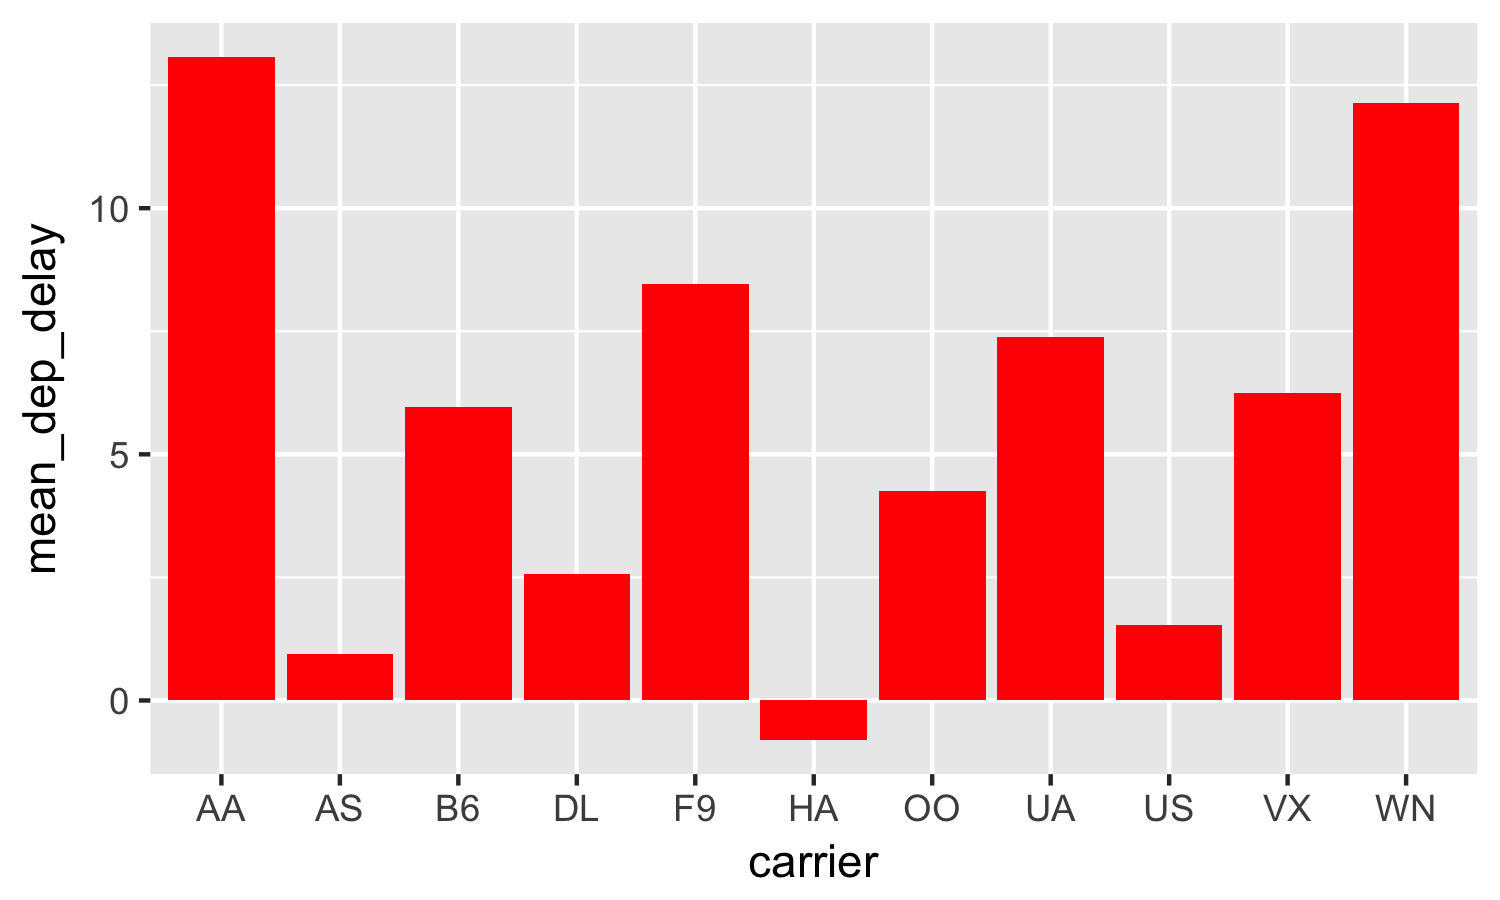
\includegraphics[scale = 0.3,angle = 0]{figure/delays.png}
  \caption[Mean Delays by Airline]{\normalsize{Mean Delays by Airline}}
  \label{fig:delays}
  \end{figure}
  
  A table linking these carrier codes to airline names is available at
  \url{https://github.com/ismayc/pnwflights14/blob/master/data/airlines.csv}.
  
  \clearpage
  
  Next, we will explore the use of the \texttt{scale} parameter which can
  be used to shrink or expand an image. Here we use the mathematical graph
  stored in the ``subdivision.pdf'' file. Note that we didn't specify the
  \texttt{caption\ =} or \texttt{label\ =} here, but we could have.
  
  \begin{Shaded}
  \begin{Highlighting}[]
  \KeywordTok{label}\NormalTok{(}\StringTok{"figure/subdivision.pdf"}\NormalTok{, }\StringTok{"Subdiv. graph"}\NormalTok{, }\StringTok{"subd"}\NormalTok{, }
        \DataTypeTok{scale =} \FloatTok{0.75}\NormalTok{)}
  \end{Highlighting}
  \end{Shaded}
  
  \begin{figure}[htbp]
  \centering
  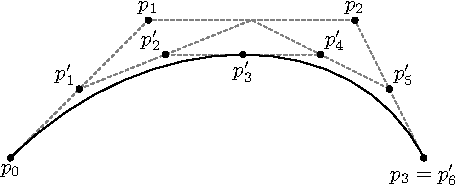
\includegraphics[scale = 0.75,angle = 0]{figure/subdivision.pdf}
  \caption[Subdiv. graph]{\normalsize{Subdiv. graph}}
  \label{fig:subd}
  \end{figure}
  
  Here is a reference to this image: \autoref{fig:subd}. (Move this around
  throughout the document as you wish.)
  
  \subsubsection{More Figure Stuff}\label{more-figure-stuff}
  
  Lastly, we will explore how to rotate figures using the \texttt{angle}
  parameter.
  
  \begin{Shaded}
  \begin{Highlighting}[]
  \KeywordTok{label}\NormalTok{(}\StringTok{"figure/subdivision.pdf"}\NormalTok{, }
        \StringTok{"A Larger Figure, Flipped Upside Down"}\NormalTok{, }
        \DataTypeTok{scale =} \FloatTok{1.5}\NormalTok{,}
        \DataTypeTok{angle =} \DecValTok{180}\NormalTok{,}
        \DataTypeTok{label =} \StringTok{"subd2"}\NormalTok{)}
  \end{Highlighting}
  \end{Shaded}
  
  \begin{figure}[htbp]
  \centering
  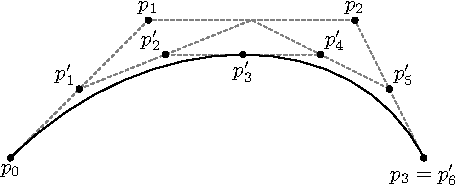
\includegraphics[scale = 1.5,angle = 180]{figure/subdivision.pdf}
  \caption[A Larger Figure, Flipped Upside Down]{\normalsize{A Larger Figure, Flipped Upside Down}}
  \label{fig:subd2}
  \end{figure}
  
  As another example, here is a reference to this figure:
  \autoref{fig:subd2}.
  
  \subsubsection{Common Modifications}\label{common-modifications}
  
  The following figure features the more popular changes thesis students
  want to their figures. We can add math to the caption that displays
  below the picture, specify the size of our caption to display below the
  figure (list of sizes available at this
  \href{http://www.emerson.emory.edu/services/latex/latex_169.html\#SEC169}{link}),
  and also specify that a different caption \texttt{alt.cap} be what
  appears in the Table of Figures for this figure.
  
  If you'd like to make further tweaks to figures, you might need to
  invoke some \LaTeX~code.
  
  \begin{Shaded}
  \begin{Highlighting}[]
  \KeywordTok{label}\NormalTok{(}\StringTok{"figure/subdivision.pdf"}\NormalTok{, }
        \DataTypeTok{caption =} \StringTok{"Subdivision of arc segments"}\NormalTok{,}
        \DataTypeTok{alt.cap =} \StringTok{"You can see that $p_3 = p_6^}\CharTok{\textbackslash{}\textbackslash{}}\StringTok{prime$"}\NormalTok{,}
        \DataTypeTok{cap.size =} \StringTok{"footnotesize"}\NormalTok{,}
        \DataTypeTok{label =} \StringTok{"subd3"}\NormalTok{)}
  \end{Highlighting}
  \end{Shaded}
  
  \begin{figure}[htbp]
  \centering
  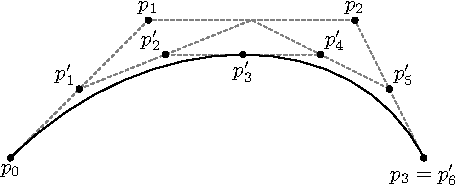
\includegraphics[scale = 1,angle = 0]{figure/subdivision.pdf}
  \caption[Subdivision of arc segments]{\footnotesize{You can see that $p_3 = p_6^\prime$}}
  \label{fig:subd3}
  \end{figure}
  
  \section{Footnotes and Endnotes}\label{footnotes-and-endnotes}
  
  You might want to footnote something.\footnote{footnote text} The
  footnote will be in a smaller font and placed appropriately. Endnotes
  work in much the same way.
  
  \section{Bibliographies}\label{bibliographies}
  
  Of course you will need to cite things, and you will probably accumulate
  an armful of sources. There are a variety of tools available for
  creating a bibliography database (stored with the .bib extension). In
  addition to BibTeX suggested below, you may want to consider using the
  free and easy-to-use tool called Zotero.
  
  \emph{R Markdown} uses \emph{pandoc} (\url{http://pandoc.org/}) to build
  its bibliographies. One nice caveat of this is that you won't have to do
  a second compile to load in references as standard \LaTeX~requires. To
  cite references in your thesis (after creating your bibliography
  database), place the reference name inside square brackets and precede
  it by the ``at'' symbol. For example, here's a reference to a book about
  worrying: (Molina \& Borkovec, 1994). This \texttt{Molina1994} entry
  appears in a file called \texttt{thesis.bib} in the \texttt{bib} folder.
  This bibliography database file was created by a program called BibTeX.
  You can call this file something else if you like (look at the YAML
  header in the main .Rmd file) and, by default, is to placed in the
  \texttt{bib} folder.
  
  For more information about BibTeX and bibliographies, see Reed College's
  CUS site (\url{http://web.reed.edu/cis/help/latex/index.html})\footnote{Reed~College
    (2007)}. There are three pages on this topic: \emph{bibtex} (which
  talks about using BibTeX, at
  \url{http://web.reed.edu/cis/help/latex/bibtex.html}),
  \emph{bibtexstyles} (about how to find and use the bibliography style
  that best suits your needs, at
  \url{http://web.reed.edu/cis/help/latex/bibtexstyles.html}) and
  \emph{bibman} (which covers how to make and maintain a bibliography by
  hand, without BibTeX, at
  \url{http://web.reed.edu/cis/help/latex/bibman.html}). The last page
  will not be useful unless you have only a few sources.
  
  If you look at the YAML header at the top of the main .Rmd file you can
  see that we can specify the style of the bibliography by referencing the
  appropriate csl file. You can download a variety of different style
  files at \url{https://www.zotero.org/styles}. Make sure to download the
  file into the csl folder.
  
  \paragraph{Tips for Bibliographies}\label{tips-for-bibliographies}
  
  \begin{itemize}
  \tightlist
  \item
    Like with thesis formatting, the sooner you start compiling your
    bibliography for something as large as thesis, the better. Typing in
    source after source is mind-numbing enough; do you really want to do
    it for hours on end in late April? Think of it as procrastination.
  \item
    The cite key (a citation's label) needs to be unique from the other
    entries.
  \item
    When you have more than one author or editor, you need to separate
    each author's name by the word ``and'' e.g.
    \texttt{Author\ =\ \{Noble,\ Sam\ and\ Youngberg,\ Jessica\},}.
  \item
    Bibliographies made using BibTeX (whether manually or using a manager)
    accept \LaTeX~markup, so you can italicize and add symbols as
    necessary.
  \item
    To force capitalization in an article title or where all lowercase is
    generally used, bracket the capital letter in curly braces.
  \end{itemize}
  
  \chapter*{Conclusion}\label{conclusion}
  \addcontentsline{toc}{chapter}{Conclusion}
  
  \setcounter{chapter}{4} \setcounter{section}{0}
  
  If we don't want Conclusion to have a chapter number next to it, we can
  add the \texttt{\{.unnumbered\}} attribute. This has an unintended
  consequence of the sections being labeled as 3.6 for example though
  instead of 4.1. The \LaTeX~commands immediately following the Conclusion
  declaration get things back on track.
  
  \subsubsection{More info}\label{more-info}
  
  And here's some other random info: the first paragraph after a chapter
  title or section head \emph{shouldn't be} indented, because indents are
  to tell the reader that you're starting a new paragraph. Since that's
  obvious after a chapter or section title, proper typesetting doesn't add
  an indent there.
  
  \appendix
  
  \singlespacing
  
  \chapter{The First Appendix}\label{the-first-appendix}
  
  This first appendix includes all of the R chunks of code that were
  hidden throughout the document (using the \texttt{include\ =\ FALSE}
  chunk tag) to help with readibility and/or setup.
  
  \subsubsection{In the main Rmd file:}\label{in-the-main-rmd-file}
  
  \begin{Shaded}
  \begin{Highlighting}[]
  \CommentTok{# This chunk ensures that the acstats package is}
  \CommentTok{# installed and loaded. This acstats package includes}
  \CommentTok{# the template files for the thesis and also two functions}
  \CommentTok{# used for labeling and referencing}
  \ControlFlowTok{if}\NormalTok{(}\OperatorTok{!}\KeywordTok{require}\NormalTok{(devtools))}
    \KeywordTok{install.packages}\NormalTok{(}\StringTok{"devtools"}\NormalTok{, }\DataTypeTok{repos =} \StringTok{"http://cran.rstudio.com"}\NormalTok{)}
  \ControlFlowTok{if}\NormalTok{(}\OperatorTok{!}\KeywordTok{require}\NormalTok{(acstats))\{}
    \KeywordTok{library}\NormalTok{(devtools)}
  \NormalTok{  devtools}\OperatorTok{::}\KeywordTok{install_github}\NormalTok{(}\StringTok{"Amherst-Statistics/acstats"}\NormalTok{)}
  \NormalTok{\}}
  \KeywordTok{library}\NormalTok{(acstats)}
  \KeywordTok{library}\NormalTok{(knitr)}
  \KeywordTok{library}\NormalTok{(readr)}
  \KeywordTok{library}\NormalTok{(fastICA)}
  \KeywordTok{library}\NormalTok{(ica)}
  \KeywordTok{library}\NormalTok{(gridExtra)}
  \end{Highlighting}
  \end{Shaded}
  
  \subsubsection{\texorpdfstring{In
  \protect\hyperlink{ref_labels}{}:}{In :}}\label{in}
  
  \begin{Shaded}
  \begin{Highlighting}[]
  \CommentTok{# This chunk ensures that the acstats package is}
  \CommentTok{# installed and loaded. This acstats package includes}
  \CommentTok{# the template files for the thesis and also two functions}
  \CommentTok{# used for labeling and referencing}
  \ControlFlowTok{if}\NormalTok{(}\OperatorTok{!}\KeywordTok{require}\NormalTok{(devtools))}
    \KeywordTok{install.packages}\NormalTok{(}\StringTok{"devtools"}\NormalTok{, }\DataTypeTok{repos =} \StringTok{"http://cran.rstudio.com"}\NormalTok{)}
  \ControlFlowTok{if}\NormalTok{(}\OperatorTok{!}\KeywordTok{require}\NormalTok{(dplyr))}
      \KeywordTok{install.packages}\NormalTok{(}\StringTok{"dplyr"}\NormalTok{, }\DataTypeTok{repos =} \StringTok{"http://cran.rstudio.com"}\NormalTok{)}
  \ControlFlowTok{if}\NormalTok{(}\OperatorTok{!}\KeywordTok{require}\NormalTok{(ggplot2))}
      \KeywordTok{install.packages}\NormalTok{(}\StringTok{"ggplot2"}\NormalTok{, }\DataTypeTok{repos =} \StringTok{"http://cran.rstudio.com"}\NormalTok{)}
  \ControlFlowTok{if}\NormalTok{(}\OperatorTok{!}\KeywordTok{require}\NormalTok{(acstats))\{}
    \KeywordTok{library}\NormalTok{(devtools)}
  \NormalTok{  devtools}\OperatorTok{::}\KeywordTok{install_github}\NormalTok{(}\StringTok{"Amherst-Statistics/acstats"}\NormalTok{)}
  \NormalTok{  \}}
  \KeywordTok{library}\NormalTok{(acstats)}
  \NormalTok{flights <-}\StringTok{ }\KeywordTok{read.csv}\NormalTok{(}\StringTok{"data/flights.csv"}\NormalTok{)}
  \end{Highlighting}
  \end{Shaded}
  
  \chapter{The Second Appendix, for
  Fun}\label{the-second-appendix-for-fun}
  
  \backmatter
  
  \chapter{References}\label{references}
  
  \noindent
  
  \setlength{\parindent}{-0.20in} \setlength{\leftskip}{0.20in}
  \setlength{\parskip}{8pt}
  
  \hypertarget{refs}{}
  \hypertarget{ref-icaR}{}
  Helwig, N. E. (2015, August). Independent component analysis.
  \emph{``Proceedings of'' SIGGRAPH 2000}. Retrieved from
  \url{https://cran.r-project.org/web/packages/ica/ica.pdf}
  
  \hypertarget{ref-Oja2000}{}
  Hyvärinen, A., \& Oja, E. (2000). Independent component analysis:
  Algorithms and applications. \emph{``'Independent Component Analysis:
  Algorithms and Applications' Neural Netw. 200}, 411--30.
  
  \hypertarget{ref-izenman2003}{}
  Izenman, A. J. (2003). What is independent component analysis?
  
  \hypertarget{ref-fastICA}{}
  J L Marchini \textless{}marchini@stats.ox.ac.uk\textgreater{}, C. H.
  \textless{}. r, \& \textless{}ripley@stats.ox.ac.uk\textgreater{}, B. D.
  R. (2017, June). FastICA algorithms to perform ica and projection
  pursuit. Retrieved from
  \url{https://cran.r-project.org/web/packages/fastICA/fastICA.pdf}
  
  \hypertarget{ref-Molina1994}{}
  Molina, S. T., \& Borkovec, T. D. (1994). The Penn State worry
  questionnaire: Psychometric properties and associated characteristics.
  In G. C. L. Davey \& F. Tallis (Eds.), \emph{Worrying: Perspectives on
  theory, assessment and treatment} (pp. 265--283). New York: Wiley.
  
  \hypertarget{ref-puigt2011}{}
  Puigt, M. (2011). \emph{A very short introduction to blind source
  separation}. Heraklion, Crete, Greece: Foundation for Research;
  Technology -- Hellas Institute of Computer Science.
  
  \hypertarget{ref-reedweb2007}{}
  Reed~College. (2007, March). LaTeX your document. Retrieved from
  \url{http://web.reed.edu/cis/help/LaTeX/index.html}


  % Index?

\end{document}

